\documentclass[12pt]{article}
\usepackage{amsmath}
\usepackage{enumerate}
\usepackage{mathrsfs} 
\usepackage{amsthm}
\usepackage{amsfonts}
\usepackage{amssymb}
\usepackage{latexsym} 
%\usepackage{epsfig}
%\usepackage{graphicx}
%\usepackage[dvips]{graphicx}
\usepackage{tikz}
\usepackage{tikz-cd}
\usepackage{url}


\usepackage[matrix,tips,graph,curve]{xy}

\newcommand{\mnote}[1]{${}^*$\marginpar{\footnotesize ${}^*$#1}}
\linespread{1.065}

\makeatletter

\setlength\@tempdima  {5.5in}
\addtolength\@tempdima {-\textwidth}
\addtolength\hoffset{-0.5\@tempdima}
\setlength{\textwidth}{5.5in}
\setlength{\textheight}{8.75in}
\addtolength\voffset{-0.625in}

\makeatother

\makeatletter 
\@addtoreset{equation}{section}
\makeatother


\renewcommand{\theequation}{\thesection.\arabic{equation}}

\theoremstyle{plain}
\newtheorem{theorem}[equation]{Theorem}
\newtheorem{corollary}[equation]{Corollary}
\newtheorem{conjecture}[equation]{Conjecture}
\newtheorem{lemma}[equation]{Lemma}
\newtheorem{proposition}[equation]{Proposition}
\theoremstyle{definition}
\newtheorem{definition}[equation]{Definition}
\newtheorem{definitions}[equation]{Definitions}
%\theoremstyle{remark}

\newtheorem{remark}[equation]{Remark}
\newtheorem{remarks}[equation]{Remarks}
\newtheorem{exercise}[equation]{Exercise}
\newtheorem{example}[equation]{Example}
\newtheorem{examples}[equation]{Examples}
\newtheorem{notation}[equation]{Notation}
\newtheorem{question}[equation]{Question}
\newtheorem{assumption}[equation]{Assumption}
\newtheorem*{claim}{Claim}
\newtheorem{answer}[equation]{Answer}
%%%%%% letters %%%%

\newcommand{\fa}{\mathfrak{a}}
\newcommand{\fb}{\mathfrak{b}}
\newcommand{\fm}{\mathfrak{m}}
\newcommand{\fp}{\mathfrak{p}}
\newcommand{\fq}{\mathfrak{q}}

\newcommand{\IA}{\mathbb{A}}
\newcommand{\IN}{\mathbb{N}}
\newcommand{\IF}{\mathbb{F}}
\newcommand{\IP}{\mathbb{P}}
\newcommand{\IZ}{\mathbb{Z}}

\newcommand{\sB}{\mathcal{B}}
\newcommand{\sD}{\mathcal{D}}
\newcommand{\sI}{\mathcal{I}}
\newcommand{\sO}{\mathcal{O}}
\newcommand{\sP}{\mathcal{P}}
\newcommand{\sQ}{\mathcal{Q}}
\newcommand{\sS}{\mathcal{S}}
\newcommand{\sT}{\mathcal{T}}
\newcommand{\sU}{\mathcal{U}}

\newcommand{\shF}{\mathscr{F}}
\newcommand{\shG}{\mathscr{G}}
%%%%%%% macros %%%%%

%% my definitions %%%

\newcommand{\End}{\mathrm{End}}
\newcommand{\tr}{\mathrm{tr}}
\newcommand{\Hom}{\mathrm{Hom}}
\newcommand{\Aut}{\mathrm{Aut}}
\newcommand{\Trace}{\mathrm{Trace}\,}
\newcommand{\rank}{\mathrm{rank}}
\renewcommand{\deg}{\mathrm{deg}\,}
\newcommand{\Spec}{\rm Spec\,}
\newcommand{\Proj}{\rm Proj\,}
\newcommand{\Sym}{\mathrm{Sym \,}}
\newcommand{\Span}{\mathrm{Span \,}}
\renewcommand\dim{{\rm dim\,}}
\newcommand{\codim}{{\rm codim\,}}
\renewcommand\det{{\rm det\,}}
\newcommand{\im}{{\rm Im\,}}


\newcommand\iso{{\, \simeq \,}} 
\newcommand\tensor{{\otimes}}
\newcommand\Tensor{{\bigotimes}} 
\newcommand\union{\bigcup} 
\newcommand\onehalf{\frac{1}{2}}
\newcommand\trivial{{\mathbb I}}
\newcommand\wb{\overline}

%%%%%Delimiters%%%%

\newcommand{\<}{\langle}
\renewcommand{\>}{\rangle}

%\renewcommand{\(}{\left(}
%\renewcommand{\)}{\right)}


%%%% Different kind of derivatives %%%%%

\newcommand{\delbar}{\bar{\partial}}
\newcommand{\pdu}{\frac{\partial}{\partial u}}
%\newcommand{\pd}[1][2]{\frac{\partial #1}{\partial #2}}

%%%%% Arrows %%%%%
\newcommand{\induce}{\rightsquigarrow}
\newcommand{\into}{\hookrightarrow}
\newcommand{\onto}{\twoheadrightarrow}
\newcommand{\tto}{\longmapsto}
\def\llra{\longleftrightarrow}
\def\wt{\widetilde}
\def\wtilde{\widetilde}
\def\what{\widehat}
\def\bf{\textbf}
\def\it{\textit}
%%%%%%%%%%%%%%%%%%% Ziquan's definitions %%%%%%%%%%%%%%%%%%%%
\newcommand{\Ann}{\mathrm{Ann}}
\newcommand{\height}{\mathrm{height \,}}
\newcommand{\Div}{\mathrm{Div}}
\newcommand{\sE}{\mathcal{E}}
\newcommand{\p}{\partial}
\newcommand{\Ohm}{\Omega}
\newcommand{\w}{\omega}
\newcommand{\sing}{\mathrm{sing}}
%%%%%%%%%%%%% new definitions for the positive mass paper %%%%%%%%%

\newcommand{\sperp}{{\scriptscriptstyle \perp}}
\newcommand{\Qmed}{\mathcal{Q}_r^\mathrm{medium}}
\newcommand{\Qhigh}{\mathcal{Q}^\mathrm{high}}
\newcommand{\uppermu}{\overline{\mu}}
\newcommand{\lowermu}{\underline{\mu}}
\newcommand{\res}{\mathrm{res}}
\newcommand{\ev}{\mathrm{ev}}
\newcommand{\pr}{\mathrm{pr}}
\newcommand{\Prob}{\mathrm{Prob}}
\newcommand{\st}{\, \mathrm{ s.t. }\,}

\newcommand{\bq}{\textbf{q}}

\newcommand{\ad}{\mathrm{ad}}
\newcommand{\red}{\mathrm{red}}

\newcommand{\IC}{\mathbb{C}}
\newcommand{\grad}{\mathrm{grad}}


\newcommand{\upmu}{\overline{\mu}}

\newcommand{\yk}{\lfloor d/p \rfloor}

\newcommand{\shR}{\mathscr{R}}
\newcommand{\shC}{\mathscr{C}}

\newcommand{\sW}{\mathcal{W}}

\newcommand{\Irr}{\mathrm{Irr}}
\newcommand{\fl}[1]{\lfloor #1 \rfloor}
\newcommand*{\rom}[1]{\expandafter\@slowromancap\romannumeral #1@}


%%%%%%%%%%%%%%%%%%%%%%%

%%%%%%%%%%%%%%%%%%%%%%%%%%%%%%%%%%%%%%%%%%%%%





%
\begin{document}
%
\title{Undergraduate Senior Thesis}
\author{Ziquan Yang}
\date{\today}

\maketitle

\tableofcontents

\section{Introduction}
Let $X$ be a non-singular closed subvariety of $\IP^N$ of dimension $m$ over a ground field $\kappa$ . The classical Bertini theorem states that if $\kappa$ is algebraically closed, then for almost all hyperplanes $H$, $H \cap X$ is non-singular. More precisely, the set of all hyperplanes with this property forms an open dense subset of the complete linear system $|\sO_{\IP^N}(1)|$, considered as a projective space.  

The classical Bertini theorem is known to fail for finite fields, as Poonen demonstrated in \cite{Poonen}. However, he used the closed point sieve to show that the asymptotic density of degree $d$ hypersurfaces that intersect $X$ transversely as $d \to \infty$ is $\zeta_{X}(m + 1)^{-1}$. More precisely, if $\sS \subseteq \union_d H^0(\IP^n, \sO(d))$, the asymptotic density of $\sS$, denoted by $\mu(\sS)$, is defined by 
$$ \mu(\sS) : = \lim_{d \to \infty} \frac{\# \sS \cap H^0(\IP^n, \sO(d))}{\# H^0(\IP^n, \sO(d))}$$
if it exists, and Poonen proved the following theorem:
\begin{theorem}
Let $X$ be a smooth quasi-projective subscheme of $\IP^n$ of dimension $m \ge 0$ over $\IF_q$. Define 
$$ \sP := \{ f \in \union_{d \ge 0} H^0(\IP^n, \sO(d)) : \{ f = 0 \} \cap X \textit{ is smooth of dimension } m - 1 \}$$
Then $\mu(\sP) = \zeta_X(m + 1)^{-1}$. 
\end{theorem}

Poonen employed an analogue of the sieve method in number theory, which he called the ``closed point sieve", in the proof of the theorem. We may explain the main idea of his proof here. The condition that $\{ f = 0 \} \cap X$ is singular at a closed point $Q \in X$ amounts to $m + 1$ linear conditions on the coefficients of $f$, since if we dehomogenize $f$ in an affine chart of $\IP^n$ that contains $Q$ to obtain a regular function in the neighborhood of $Q$, then all partial derivatives of this function have to vanish. These linear conditions are over the residue field of $Q$. When $d$ is large enough, $f$ has more than $d + 1$ coefficients, the density of $f$ such that $f = 0$ intersects $X$ transversely at $Q$ is $(1 - q^{-(m + 1) \deg Q})$. In fact, let $\sP_{e}$ denote the set $\union_d \{ f \in H^0(\IP^n, \sO(d)) : \{f=0\} \cap X \textit{ is smooth at all }Q \textit{ with } \deg Q \le e \}$, it is not hard to prove that 
\begin{align*}
\mu(\sP_e) = \prod_{Q \in X : \deg Q \le e} (1 - q^{-(m + 1) \deg Q})
\end{align*}  
We may guess that $\mu(\sP) = \lim_{d \to \infty} \mu(\sP_e) = \zeta_X(m + 1)^{-1}$. Indeed, essentially what we need to do is to justify a change of the order of two limits
$$ \lim_{d \to \infty} \frac{\# \cap_{e = 1}^\infty \sP_e \cap H^0(\IP^n, \sO(d))}{\# H^0(\IP^n, \sO(d))} = \lim_{e \to \infty} \lim_{d \to \infty} \frac{\# \sP_e \cap H^0(\IP^n, \sO(d))}{\# H^0(\IP^n, \sO(d))}$$
Therefore, the only thing left is to bound the tail terms, and indeed this is the most technical part of the proof. Poonen used a very clever decoupling idea to control the error that arises from ignoring the conditions from points of high degree. 


In fact, Poonen proved a more general version of the theorem, with which he demonstrated many new results. He used it to construct counterexamples to the original hyperplane Bertini theorem when the base field is finite. He could also construct examples of space-filling and space-avoiding varieties. For example, he proved the following:

\begin{theorem}
Let $X$ be a smooth, projective, geometrically integral variety of dimension $m \ge 1$ over $\IF_q$, and let $E$ be a finite extension of $\IF_q$. Then there exists
a smooth, projective, geometrically integral curve $Y \subseteq X$ such that $Y(E) = X(E)$.
\end{theorem}

Poonen's theorem 1.1 has been generalized by Erman and Wood to semiample divisors in \cite{Wood}.  

\begin{theorem}
Let $X$ be a smooth projective variety over $\IF_q$, with a
very ample divisor $A$ and a globally generated divisor $E$. Let $\pi$ be the map given by the
complete linear series on E.
$$ \pi : X \stackrel{|E|}{\to} \IP^M $$
There exists an $n_0$, depending only on $\dim X$ and $\mathrm{char\,} \IF_q$, such that for $n \ge n_0$, the
probability of smoothness for a random $D \in |nA + dE|$ as $d \to \infty$ is given by the product of local probabilities taken over the fibers of $\pi$:
$$ \Prob(D \text{ is smooth}) = \prod_{P \in \IP^M} \Prob(D \text{ is smooth at all points of } \pi^{-1}(P)). $$
The product on the right converges, is zero only if some factor is zero, and is always non-zero for $n$ sufficiently large.
\end{theorem}

By ``probability", they mean an asymptotic probability, which is defined in the same way that Poonen defined the asymptotic density. 

This thesis studies non-singular hypersurfaces of bidegree $(3, d)$ in $\IP^1 \times \IP^1$ and $\IP^2 \times \IP^1$ over a finite field $\IF_q$. Via the second projection to $\IP^1$, these hypersurfaces can viewed as $\IP^1$-families of three collinear points and plane cubics respectively. Due to topological constraints, these families will inevitably contain some singular fibers. We may ask for the density of those families whose fibers have at worst the simplest type of singularity. We borrow techniques from \cite{Wood} to show that we can express this density as an infinite product taken over all closed points in $\IP^1$. However, we need to make some nontrivial adjustments to the sieve method to bound the error terms in our case. In particular, in the study of hypersurfaces of bidegree $(3, d)$ in $\IP^2 \times \IP^1$, we employ the basic idea of \textit{linearization}.

In \cite{expository}, Poonen proposed a principle that ``If an existence result about polynomials
or $n$-tuples of polynomials over an infinite field can be proved by dimension counting,
then a corresponding result over finite fields can be proved by the closed point sieve." Both our results conform to this principle. The author hopes that these results will be of some use to inspire the formulation of some meta-theorems that make this principle precise.  


\section{Simply Ramified Curves in $\IP^1 \times \IP^1$}
\label{simplify-ramified}
\subsection{Introduction}
Among other things, Erman and Wood showed that for fixed $n \ge 3$, over a finite field $\kappa = \IF_q$, the asymptotic probability for a randomly chosen curve in $\IP^1 \times \IP^1$ of bidegree $(n, d)$ to be non-singular is $\zeta_{\IP^1_{\IF_q}}(2)^{-1}\zeta_{\IP^1_{\IF_q}}(3)^{-1}$ as $d \to \infty$ [\cite{Wood}, Theorem 9.5].
In this section, we attempt to study ramifications of these curves with respect to the second projection $\pi: \IP^1 \times \IP^1 \to \IP^1$. When $n \ge 2, d > 1$, a non-singular curve $C$ of bidegree $(n, d)$ has genus $nd - n - d + 1 >  0$ [\cite{Hartshorne}, Chapter \uppercase\expandafter{\romannumeral3} Exercise 5.6 (c)], and hence by Riemann-Hurwitz theorem, $\pi : C \to \IP^1$ is necessarily ramified. In other words, if we view the curve $C$ as a $\IP^1$-family of three collinear points via $\pi$, then $C$ necessarily contains singular fibers.  

Nonetheless we can show that if the ground field $\kappa$ is algebraically closed, then for a sufficiently general choice of $C$, the ramification of $\pi : C \to \IP^1$ is simple. Moreover, the set of the curves with this property forms a dense subset of $|\sO_{\IP^1 \times \IP^1}(n, d)|$, viewed as a projective space. Then we borrow techniques from papers \cite{Poonen} and \cite{Wood} to show that when $\kappa = \IF_q$ with $p = \mathrm{char}\, \IF_q > 2$ and $n = 3$, the asymptotic probability for a randomly chosen curve in the divisor class $|\sO_{\IP^1 \times \IP^1}(3, d)|$ to be simply ramified with respect to $\pi$ is $\zeta_{\IP^1_{\IF_q}}(2)^{-2}$ as $d \to \infty$. 
 


\paragraph{Notation} 
Let $X$ be $\IP^1 \times \IP^1$ over a ground field $\kappa$. We label its coordinates as $((s_0, s_1), (t_0, t_1))$. $\pi : X \to \IP^1$ is the second projection. If $W \subset \IP^1$ is a finite subscheme, the fiber $\pi^{-1}(W) \subset X$ is denoted by $X_W$. Let $R_{n, d} \subseteq \kappa[s_0, s_1, t_0, t_1]$ be the set of bihomogeneous polynomials that are of degree $n$ in $s_0, s_1$ and $d$ in $t_0, t_1$. $R_{n, d}$ can be naturally identified with $H^0(\IP^1 \times \IP^1, \sO(n, d))$. For a section $f \in R_{n, d}$, the curve in $X$ cut out by $f$ is denoted by $H_f$. The fiber of $H_f$ over $P \in \IP^1$ is denoted by $(H_f)_P$. If $Q \in X$ is a closed point and $C \subseteq X$ is a curve that is non-singular at $Q$, then $e_Q(C)$ denotes the ramification degree of $C$ with respect to $\pi$. When $\kappa = \IF_q$ is finite, for a subset $\sP \subseteq \union_d R_{n, d}$, we define 
$$ \Prob(f \in \sP) := \lim_{d \to \infty}\Prob(f_d \in \sP) = \lim_{d \to \infty} \frac{\# \sP \cap R_{n, d}}{\# R_{n, d}}$$
where $f$ and $f_d$ are randomly chosen from $\union_{d} R_{n, d}$ and $R_{n, d}$ respectively. 

In general, if $Y$ is a scheme and $Q$ is a closed point in $Y$, we use $Q^{(2)}$ to denote the first-order infinitesimal neighborhood of $Q$ in $Y$. The residue field of $Q$ is denoted by $\kappa(Q)$.

\subsection{An Analogue of Bertini's Theorem} 
Given a point $f \in |\sO_X(n,d)|$, viewed as a projective space, we denote the corresponding hypersurface by $H_f$. 
\begin{theorem}
Let $n \ge 3$. When $\kappa$ is algebraically closed, then for almost all $f \in |\sO_X(n,d)|$, $H_f$ is simply ramified. More precisely, the set of sections $f \in |\sO_X(n, d)|$ for which $H_f$ is not simply ramified is contained in a proper closed subscheme of $|\sO_X(n, d)|$. 
\end{theorem} 
\begin{proof}
Recall that non-singularity is an open condition. Let $N$ denote the open subscheme that parametrizes those non-singular curves. A non-singular curve fails to be simply ramified if and only if it falls into at least one of the following two types: 

\begin{enumerate}[I.]
\item $e_Q(H_f) \ge 3$ for some $Q \in X$. 
\item $e_{Q}(H_f), e_{Q'}(H_f) \ge 2$ for some pair $Q \neq Q' \in X$ with $\pi(Q) = \pi(Q')$. 
\end{enumerate}
We may deal with them separately. \\\\
\textit{Type \uppercase\expandafter{\romannumeral1} curves}: Consider the subset $B_1 \subseteq X \times N$ consisting of all pairs $(Q, f)$ such that $Q \in X$ is a closed point and $e_Q(H_f) \ge 3$. We show that $B_1$ is the set of closed points of a closed subscheme $X \times N$, which we denote also by $B_1$. It suffices to check this locally. Without loss of generality, consider $\IA^1 \times \IA^1 \subseteq \IP^1 \times \IP^1$, where $\IA^1 \times \IA^1$ is the affine chart on which $t_1, s_1 \neq 0$. We may use affine coordinates $s := s_0/s_1$ and $t := t_0/t_1$ on $\IA^1 \times \IA^1$. Identify $R_{n, d} = H^0(X, \sO_X(n, d))$ with the dehomogenizations on $\IA^1 \times \IA^1$, so that we may write 
\begin{equation} \label{ident} f = \sum_{0 \le i \le n} \sum_{0 \le j \le d} a_{ij} s^i t^j \end{equation}
where $(a_{ij})$ is the coordinate for $f$. On $(\IA^1 \times \IA^1) \times N$, $B_1$ can be described by 
\begin{equation} f = \frac{\p f}{\p s} = \frac{\p^2 f}{\p s^2} = 0 \end{equation}
Therefore we have checked locally that $B_1$ is closed in $X \times N$. We may hence give $B_1$ a reduced induced scheme structure. Let $p_1 : B_1 \to X$ be the first projection. For each $Q$, $f(Q) = f_s(Q) = f_{ss}(Q)$ amounts to 3 linear equations on $(a_{ij})$, and these equations are clearly linearly independent. Therefore the fiber $p_1^{-1}(Q)$ is the intersection of $N$ with some projective subspace of $|\sO_X(n, d)|$ of codimension $3$. Since $\dim X = 2$, we see that $\dim B_1 = \dim |\sO_X(n, d)| - 1$. Type \uppercase\expandafter{\romannumeral1} curves are clearly contained in the image of $B_1$ under the second projection, and hence contained in a proper closed subscheme of $|\sO_X(n, d)|$. \\\\
\textit{Type \uppercase\expandafter{\romannumeral2} curves: }We perform a sieve on pairs of points in $X$, which can be parametrized by $X \times X$. Consider the subset $B_2' \subseteq X \times X \times |\sO_X(n, d)|$ of all triples $(Q', Q, f)$ such that $e_{Q}(H_f), e_{Q'}(H_f) \ge 2$ and $\pi(Q) = \pi(Q')$. Let us label the coordinates of the first copy of $X$ by $((s_0' : s_1'), (t_0' : t_1'))$ and the second one still by $((s_0 : s_1), (t_0, t_1))$. We first check that $B_2'$ is a closed subset. Without loss of generality, let $(\IA^1 \times \IA^1) \times (\IA^1 \times \IA^1) \subset X \times X$ be the affine chart where $s_1', t_1', s_1, t_1 \neq 0$, on which we use coordinates $s' = s'_0/s'_1, t' = t_0'/t_1', s = s_0/s_1, t = t_0/t_1$. On $(\IA^1 \times \IA^1) \times (\IA^1 \times \IA^1) \times |\sO_X(n, d)|$, $B_2'$ is described by 
\begin{equation} t' = t \textit{ and } f(s, t) = \frac{\p}{\p s}f(s, t) = f(s', t') = \frac{\p}{\p s'}f(s', t') = 0 \end{equation}
where we are still using the identification (\ref{ident}). For $Q$ that lies in $(\IA^1 \times \IA^1) \times (\IA^1 \times \IA^1)$, the equation $t = t'$ describes the condition that $\pi(Q)= \pi(Q')$ and the others describe the condition that $e_{Q}(H_f), e_{Q'}(H_f) \ge 2$.  Now we have checked that $B_2'$ is closed, so we may give $B_2'$ a reduced induced scheme structure. Define $$B_2 := B_2' \cap (X \times X - \Delta) \times |\sO_X(n, d)|$$ where $\Delta \subset X \times X$ is the diagonal. Let $p_1 : B_2 \to X \times X - \Delta$ be the first projection. If $(Q', Q) \in p_1(B_2) \subseteq X \times X - \Delta$ is a closed point, then $f(Q) = f(Q') = f_s(Q) = f_{s'}(Q') = 0$ amounts to $4$ linear equations on $(a_{ij})$. Since we deliberately ensured $Q \neq Q'$, these equations are linearly independent. Therefore the fiber $p_1^{-1}(Q', Q)$ is the intersection of $N$ with some projective subspace of $|\sO_X(n, d)|$ of codimension $4$. On the other hand, $\dim p_1(B_2) = 3$ since $p_1(B_2)$ is just $\{ t_0 t_1' = t_1 t_0' \} - \Delta \subseteq X \times X$, which has dimension $3$. Therefore we see that $\dim B_2 = (\dim |\sO_X(n, d)| - 4) + 3 = \dim |\sO_X(n, d)| -1$. Type \uppercase\expandafter{\romannumeral2} curves are clearly contained in the image of $B_2$ under the projection to $|\sO_X(n, d)|$, and hence contained in a proper closed subscheme of $|\sO_X(n, d)|$.
\end{proof}

\subsection{A Density Result over Finite Fields}
\begin{theorem}
\label{main}
Suppose $p = \mathrm{char } \IF_q > 2$. Let $\sD \subset \union_d R_{3,d}$ be the subset of sections $f$ such that $H_f$ is simply ramified with respect to $\pi$. Then
$$ \Prob(f \in \sD) = \zeta_{\IP^1_{\IF_q}}(2)^{-2} $$ Furthermore, the conditional probability for a randomly chosen non-singular curve of bidegree $(3, d)$ to be simply ramified is $\zeta_{\IP^1_{\IF_q}}(3)/\zeta_{\IP^1_{\IF_q}}(2)$ as $d \to \infty$. 
\end{theorem}
For convenience, we say $f \in R_{n, d}$ is ``good" at $Q \in X$, if $H_f$ is non-singular at $Q$ and $e_Q(H_f) \le 2$. If $Q \not\in H_f$, then by default $f$ is good at $Q$. Otherwise we say that $f$ is bad at $Q$. For a fixed $e_0 \in \IN$, we define 
\begin{align*}
\sP_{e_0}^{\mathrm{low}} &= \union_{d \ge 0} \{ f \in R_{3, d} : f \textit{ is good at all $Q \in X$,}\deg \pi(Q) < e_0\}\\
\sQ_{e_0}^{\mathrm{med}} &= \union_{d \ge 0} \{f \in R_{3, d} : f \textit{ is bad at some $Q$, }\deg \pi(Q) \in [e_0, \lfloor d/p \rfloor]\}\\
\sQ^{\mathrm{high}} &= \union_{d \ge 0} \{f \in R_{3, d} : f \textit{ is bad at some $Q$, }\deg \pi(Q) > d/p\}
\end{align*}
\subsubsection{Points of Low and Medium Degree}
We first do some local analysis on a fiber. Let $P \in \IP^1 = \Proj \, \IF_q[t_0, t_1]$ be a closed point. Without loss of generality, we assume $t_1 \neq 0$ at $P$ and $P$ lies in $\IA^1 = \Spec \IF_q[t]$ where $t = t_0/t_1$.   Let $\fm = (r(t))\subseteq \IF_q[t]$ be the maximal ideal corresponding to $P$, so that $\kappa(P) = \IF_q[t]/\fm, P^{(2)} = \Spec \IF_q[t]/\fm^2$ and $X_P = \IP^1_{\IF_q[t]/\fm} \subset X$. Denote the reduction map $\IF_q[t]/\fm^2 \to \IF_q[t]/\fm$ by $g \mapsto \overline{g}$. We extend it to a map $$ H^0(\IP^1_{\IF_q[t]/\fm^2}, \sO(3)) \to H^0(\IP^1_{\IF_q[t]/\fm}, \sO(3))$$ by applying $\IF_q[t]/\fm^2 \to \IF_q[t]/\fm$ to coefficients of cubic polynomials. Let $$\varphi_P : R_{3, d} \to H^0(\IP^1_{\IF_q[t]/\fm^2}, \sO(3))$$ be the restriction map. $H_f$ is non-singular at a point $Q \in X_P$ if and only if $\varphi_P(f)$ does not vanish at $Q^{(2)} \in \IP^1_{\IF_q[t]/\fm^2}$. If $H_f$ is non-singular at $Q$, then $e_Q(H_f) < 3$ if and only if $\wb{\varphi_P(f)} \in H^0(\IP^1_{\IF[t]/\fm}, \sO(3))$ does not have a zero of multiplicity $\ge 3$ at $Q$ . Therefore we can determine if $f$ is good at all points in $(H_f)_P$ by looking at the image of $f$ in $H^0(\IP^1_{\IF_q[t]/\fm^2}, \sO(3))$. This observation yields an independence result across fibers. More precisely, we have 

\begin{lemma}
\label{Low}
If $\{P_1, P_2, \cdots, P_s\}$ is a set of finitely many closed points in $\IP^1$, then for $f$ randomly chosen from $\union_d R_{3, d}$,
$$ \Prob(f \textit{ is good at all } Q \in \coprod X_{P_i}) = \prod_{i = 1}^s \Prob( f \textit{ is good at all points } Q \in (H_f)_{P_i} ) $$
In particular, we have
$$\Prob(f \in \sP_{e_0}^{\mathrm{low}})  = \prod_{\deg(P) < e_0}  \Prob( f \textit{ is good at all points } Q \in (H_f)_P ) $$
since there are only finitely many points with degree $< e_0$. 
\end{lemma}
\begin{proof} 
Let $W := \coprod P_i^{(2)}$ and $\delta := \deg W = \sum_{i = 1}^s 2 \deg P_i$. Then we have an exact sequence 
$$ 0 \to \sO_X(3, d - \delta) \to \sO_X(3, d) \to \sO_X(3, d)|_{X_W} \to 0  $$
which induces an exact sequence 
$$ H^0(X, \sO_X(3, d)) \to H^0(X_W, \sO_X(3, d)|_{X_W}) \to H^1(X, \sO_X(3, d - \delta)) $$
That $H^1(X, \sO_X(3, d - \delta)) = 0$ when $d \ge \delta$ follows from the isomorphism $H^1(X, \sO(a, b)) \cong H^1(X, \sO_X(-2-a, -2-b))$ given by Serre duality and the fact that $H^1(X, \sO_X(a, b)) = 0$ when $a, b < 0$ [\cite{Hartshorne}, Chapter \uppercase\expandafter{\romannumeral3} Exercise 5.6 (a)].
Therefore the restriction map
\begin{align*}
R_{3, d} = H^0(\IP^1 \times \IP^1, \sO(3, d)) \to H^0(X_W, \sO_X(3, d)|_{X_W}) \cong \prod_{i = 1}^s H^0(X_{P_i^{(2)}}, \sO(3))
\end{align*}
is surjective for $ d \ge \sum_i 2 \deg P_i$. This surjectivity, together with our observation that whether $f$ is good at all $Q \in (H_f)_{P_i}$ is completely determined by $\varphi_{P_i}(f) \in H^0(\IP^1_{P_i^{(2)}}, \sO(3))$, implies that when $d \ge \delta$, we have 
$$ \frac{\# R_{3, d} \cap \sP_{e_0}^{\mathrm{low}}}{\# R_{3, d}} = \prod_{i = 1}^s \frac{\# \varphi_{P_i}(\{ f \in R_{3, d} : f \textit{ is good at all }Q \in X_{P_i} \})}{\# H^0(X_{P^{(2)}_i}, \sO(3))} $$
The lemma follows by taking $d \to \infty$ on both sides. 
\end{proof}
Before proceeding we make the following convention: A pair $(F_1, F_2) \in H^0(\IP^1_{\IF_q[t]/\fm}, \sO(3))^2$ is said to be \textit{bad} if it falls in one of the following 3 types:
\begin{enumerate}
\item $F_1$ has a root of multiplicity $\ge 2$ at a point where $F_2$ also vanishes. 
\item $F_1$ has a root of multiplicity $3$ at a point where $F_2$ does not vanish. 
\item $F_1 \equiv 0$.
\end{enumerate}
Otherwise, the pair is said to be \textit{good}.
Let $\, \wt{} : \IF_q[t]/\fm \to \IF_q[t]/\fm^2$ be a $\IF_q$-linear map that is a section to the previously defined reduction map $\IF_q[t]/\fm^2 \to \IF_q[t]/\fm$. We extend it to a map $H^0(\IP^1_{\IF_q[t]/\fm^2}, \sO(3)) \to H^0(\IP^1_{\IF_q[t]/\fm}, \sO(3))$ in the same way we extended the reduction map. Then we have the following:
\begin{lemma} 
\label{pair}
The $\IF_q$-linear map 
$$ H^0(\IP^1_{\IF_q[t]/\fm}, \sO(3))^2 \to H^0(\IP^1_{\IF_q[t]/\fm^2}, \sO(3)) $$
given by $(F_1, F_2) \mapsto \wt{F}_1 + r(t)F_2$ is a bijection. Moreover, $f \in R_{3, d}$ is ``good" at all points $Q \in \pi^{-1}(P)$ if and only if $\varphi_P(f)$ corresponds to a good pair. 
\end{lemma}
\begin{proof}
The map $F \mapsto ( \wb{F}, (F - \wt{\wb{F}})/r(t))$ is an inverse to the map given in the lemma. Let $(F_1, F_2)$ be the pair corresponding to $\varphi_P(f)$. $\varphi_P(f)$ vanishes on $Q^{(2)}$, i.e. $H_f$ is singular at $Q$, if and only if $Q$ is a double root of $F_1$ and a root to $F_2$. Similarly, if $H_f$ is non-singular at $Q$, then $e_Q(H_f) \ge 3$ if and only if $Q$ is root to $F_1$ of multiplicity $\ge 3$. 
\end{proof}

\begin{lemma}
\label{count}
Let $e:= \deg P$. The density of good pairs in $H^0(\IP^1_{\kappa(P)}, \sO(3))^2$ is 
$$ (1 - q^{-2e})^{2} $$
\end{lemma}
\begin{proof}
We first count type 1 pairs. Let $Q \in \IP^1_{\IF_q[t]/\fm} = \IP^1_{\IF_{q^e}}$ be the point that is a double root to $F_1$ and a root to $F_2$. Note that $\deg Q = 1$. $F_1$ is fixed up to rescaling by $\IF_{q^e}^*$ after we choose a third root, which can be any point of degree $1$. Therefore there are $(q^e + 1)(q^e - 1)$ choices for $F_1$, where $(q^e + 1)$ is the number of all possible choices for the third root. The probability that $F_2$ vanishes at $Q$ as well is $q^{-e}$, so we have $q^{4e} q^{-e} = q^{3e}$ choices for $F_2$. Since we have $(q^e + 1)$ choices for $Q$, there are $q^{3e}(q^e + 1)^2(q^e - 1)$ type 1 pairs. 

To count type 2 pairs, let $Q \in \IP^1_{\IF_{q^e}}$ be the triple root to $F_1$. Again there are $q^e + 1$ choices. At each $Q$, there are $(q^e -1)$ homogeneous polynomials of degree $3$ which have $Q$ as a triple root, since the leading coefficient will uniquely determine such a polynomial. We have $q^{4e} - q^{3e}$ choices for $F_2$. In total there are $ (q^e + 1)(q^e - 1)(q^{4e} - q^{3e})$
pairs of type 2. 

Finally when $F_1 = 0$, $F_2$ can be anything, so we have $q^{4e}$ type 3 pairs.
Therefore the density of good pairs is 
$$ 1 - q^{-8e}(q^{3e}(q^e + 1)^2(q^e - 1) + (q^e + 1)(q^e - 1)(q^{4e} - q^{3e}) + q^{4e}) = (1 - q^{-2e})^2 $$ 
\end{proof}



\begin{lemma}
\label{Medium}
$$\lim_{e_0 \to \infty} \Prob( f \in  \sQ_{e_0}^{\mathrm{med}}) = 0 $$
\end{lemma}
\begin{proof}
By definition, 
$$ \Prob( f \in  \sQ_{e_0}^{\mathrm{med}}) = \lim_{d \to \infty} \Prob(f_d \in \sQ_{e_0}^{\mathrm{med}})$$
for $f_d$ randomly chosen from $R_{3, d}$. It suffices to show that $\Prob(f_d \in \sQ_{e_0}^{\mathrm{med}})$ is universally bounded by $O(q^{-e_0})$, where the implied constant is independent of $d$ or $e_0$. 

Let $P$ be a point of degree $e \le \lfloor d/p \rfloor$ on $\IP^1$. By the proof of Lemma~\ref{Low}, the restriction map $R_{3, d} \to H^0(X_{P^{(2)}}, \sO(3))$ is surjective since $p > 2$ and $e < \lfloor d/p \rfloor < d/2$. Lemma~\ref{pair} and Lemma~\ref{count} hence imply that probability that $f_d$ is ``bad" at some point in the fiber $X_P$ is $1 - (1 - q^{-2e})^2 < 2q^{-2e}$. 
\begin{align*}
\Prob(f_d \in \sQ_{e_0}^{\mathrm{med}}) &\le \sum_{e = e_0}^{\lfloor d/p \rfloor} (\text{number of points of degree $e$ in $\IP^1$})(2q^{-2e}) \\
&\le 2 \sum_{e = e_0}^{\lfloor d/p \rfloor}(q^{e} + 1) q^{-2e} = O(\frac{q^{-e_0}}{1 - q^{-1}}) = O(q^{-e_0})
\end{align*} 
\end{proof}

\subsubsection{Points of High Degree}
\begin{lemma}
\label{highprep}
Let $W \subseteq \IA^M \times \IA^1$ be a closed subscheme. Let $t$ be the coordinate for $\IA^1$. Denote by $A_{0, d} = \IF_q[t]_{\le d}$ the set of polynomials that are of degree $\le d$ in $t$. Let $\pi : \IA^M \times \IA^1 \to \IA^1$ be second projection. Consider the restriction map 
$$ \varphi_W : A_{0, d} \to H^0(W, \sO_W) $$
If $W$ contains a closed point $Q$ such that $\deg \pi(Q) \ge j$, then $\# \{ \im \varphi_W \} \ge q^{\min(d + 1, j)}$. 
\end{lemma}
\begin{proof}
If $\dim \pi(W) = 1$, then $t$, and hence all zero polynomials in $t$, does not vanish identically on $W$. Therefore $\varphi_W$ is injective, and $\# \{ \im \varphi_W \} = q^{d + 1}$. 
Now suppose $\dim \pi(W) = 0$. Note that $\varphi_W$ factors as
$$ A_{0, d} = \IF_q[t]_{\le d} \stackrel{\psi_W}{\to} H^0(\pi(W), \sO_{\pi(W)}) \stackrel{\pi^\#}{\to} H^0(W, \sO_W) $$ 
Since the pull back map $\pi^\#$ is injective, it suffices to bound $\# \{\im \psi_W \}$. Let $P = \pi(Q)$. Suppose $P = \Spec \IF_q[t]/(r(t)) \subset \IA^1$. Note that $\deg r(t) \ge j$ since by assumption $\deg P \ge j$. The composition 
$$ \IF_q[t]_{\le d} \to H^0(\pi(W), \sO_{\pi(W)}) \to \kappa(P) $$
is nothing but the natural map $\IF_q[t]_{\le d} \to \IF_q[t]/r(t)$. Therefore 
$$ \#\{ \im(\IF_q[t]_{\le d} \to \kappa(P)) \} = q^{\min(d + 1, j)}  \le \# \{\im \psi_W \}$$
\end{proof}

We use the following lemma to bound the probability that a randomly chosen $f \in R_{3, d}$ is bad at some point $Q$ with $\pi(Q)$ has high degree $(> \lfloor d/p \rfloor)$. Therefore the following lemma is to be applied with $j = \lfloor d/p \rfloor$. 
\begin{lemma}
\label{prep}
Let $j > 2$ be an integer and $U \subseteq X$ be an open subscheme. For a randomly chosen $f \in R_{3, d}$, the probability that there exists a point $Q \in U$ with $\deg \pi(Q) \ge j$ such that $H_f$ is non-singular at $Q$ but $e_{Q}(H_f) \ge 3$ or $H_f$ is singular at $Q$ is at most 
$$ O(d^2 q^{- \min(\lfloor d/p \rfloor + 1, j)}) $$
\end{lemma}
\begin{proof}
Among all $U$, the lemma is clearly strongest when $U = X$. Since $\IP^1 \times \IP^1$ can be covered by $4$ affine charts $\IA^1 \times \IA^1$, we reduce to proving the lemma for all $\IA^1 \times \IA^1$.  

Without loss of generality, we may assume $s_1 \neq 0, t_1 \neq 0$ on $U = \IA^1 \times \IA^1$ and work with coordinates $s = s_0/s_1, t = t_0/t_1$. Let $A_{n, d} \subseteq \IF_q[s, t] = H^0(U, \sO_U)$ be the polynomials that are of degree $\le n$ in $s$ and $\le d$ in $t$. Clearly by dehomogenizing sections in $R_{3, d}$, we have a natural identification $R_{3, d} = A_{3, d}$. Accordingly, we replace $H_f$ by $H_f \cap \IA^1 \times \IA^1$. We call a closed point $Q \in \IA^1 \times \IA^1$ \textit{admissible} if $\deg \pi(Q) \ge j$ and a subscheme $W \subseteq \IA^1 \times \IA^1$ \textit{admissible} if it contains an admissible point. By $(W)_{\mathrm{ad}}$ we denote the union of admissible irreducible components of $(W)_{\mathrm{red}}$. 

We first deal with the probability that for a randomly chosen $f \in A_{3, d}$, $e_Q(H_f) \ge 3$ at some admissible $Q \in \IA^1 \times \IA^1$, which happens only if \begin{equation} \label{ramify} f(Q) = f_s(Q) = f_{ss}(Q) = 0 \end{equation}  

Define subschemes $W_2 = \{f_{ss} = 0 \}, W_1 = W_2 \cap \{ f_s = 0 \}$ and $W_0 = W_1 \cap \{ f = 0 \}$ in $\IA^1 \times \IA^1$. We reduce the problem to bounding the probability that for a randomly chosen $f \in A_{3, d}$, $W_0$ contains an admissible point.  

Following Poonen's idea [\cite{Poonen}, Proof of Lemma 2.6], we write $f$ is such a way so that the first and second order partial derivatives with respect to $s$ are largely independent. If $f_0 \in A_{3, d}$ and $g_1, g_2, h \in A_{0, \lfloor d/p \rfloor}$ are selected uniformly and independently at random, then the distribution of 
$$ f = f_0 + g_1^p s^2 + g_2^p s + h^p $$
is uniform over $A_{3, d}$. 
Direct computation shows that 
\begin{align*}
f_s &= f_{0, s} + 2 g_1^p s + g_2^p\\
f_{ss} &= f_{0, ss} + 2 g_1^p 
\end{align*} 
Note that $W_2$ depends only on the choice of $f_0, g_1$ and $W_1$ only on $f_0, g_1, g_2$.  Let $E$ denote the event that 
\begin{enumerate}[a.]
\item $\dim (W_1)_{\ad} = 0$  
\item $f$ does not vanish identically on any irreducible component of $(W_1)_{\ad}$. 
\end{enumerate} 
Clearly if $E$ holds for $f$, then $W_0$ does not contain any admissible point. Therefore it suffices to show that for a randomly chosen $f \in A_{3, d}$, 
$$ \Prob(E) = 1 - O(d^2 q^{- \min(\lfloor d/p \rfloor + 1, j)})  $$
as $d \to \infty$. Now we bound $\Prob(E)$ in three steps: \\\\
\textit{Step 1: }Conditioned on a choice of $f_0$, the probability that $\dim W_2 = 2$ is at most $q^{- (\lfloor d/p \rfloor + 1)}$, since $\dim W_2 = 2$ if and only if $g_1^p = - f_{0, ss}/2$, for which there is at most one choice of $g_1$. \\\\
\textit{Step 2: }Conditioned on a choice of $f_0$ and $g_1$ such that $\dim W_2 = 1$, the probability that $\dim (W_1)_{\mathrm{ad}} = 1$ is at most $O(d q^{- \min(\lfloor d/p \rfloor + 1, j)})$. Let $V_1, \cdots, V_\ell$ be all the irreducible component of $(W_2)_{\mathrm{red}}$. Viewing $\IP^1 \times \IP^1$ as a subscheme of $\IP^3$ via Segre embedding, we may apply B{\'e}zout's theorem to obtain that $\ell = O(d)$. $\dim (W_1)_{\ad} = 1$ if and only if $f_s$ vanishes identically on $V_i$ for some $i$. We need to bound the set
$$ G^{\mathrm{bad}}_i = \{ g_2 \in A_{0, \lfloor d/p \rfloor} : f_{0, s} + 2 g_1^p s + g_2^p \textit{ vanishes identically on }V_i \} $$
If $g, g' \in G^{\mathrm{bad}}_i$, then $g - g'$ vanishes identically on $V_i$. Therefore $G^{\mathrm{bad}}_i$ is a coset of $\ker \varphi_i$, where $\varphi_i$ is the $\IF_q$-linear restriction map $A_{0, \lfloor d/p \rfloor} \to H^0(V_i, \sO_{V_i})$. Now we apply Lemma~\ref{highprep} to obtain that $\# \{ \im \varphi_i \} \ge q^{\min(\lfloor d/p \rfloor + 1, j)}$. This means the probability that $f_s$ vanishes identically on $V_i$ is
$$\Prob(g_2 \in G^{\mathrm{bad}}_i) = \frac{\# G^{\mathrm{bad}}_i}{\# A_{0, \lfloor d/p \rfloor}} \le q^{- \min(\lfloor d/p \rfloor + 1, j)}$$
Since there are $\ell = O(d)$ many $V_i$'s, the probability that $f_s$ vanishes identically on any of them is bounded by $O(d q^{- \min(\lfloor d/p \rfloor + 1, j)})$ as claimed. \\\\
\textit{Step 3: }Conditioned on a choice of $f_0, g_1$ and $g_2$ such that $\dim (W_1)_{\mathrm{ad}} = 0$, the probability that $(W_0)_{\mathrm{ad}} \neq \emptyset$ is at most $O(d^2 q^{- \min(\lfloor d/p \rfloor + 1, j)})$. Let $Q_1, Q_2, \cdots, Q_{\ell'}$ be all irreducible components of $(W_1)_{\mathrm{ad}}$. Since $W_1$ is cut out by $f_{s}$ and $f_{ss}$, again by considering the Segre embedding $\IP^1 \times \IP^1 \into \IP^3$, we obtain from B{\'e}zout's theorem $\ell' = O(d^2)$. Since $\pi(Q_i) \ge j$ by assumption, we may apply Lemma~\ref{highprep} again obtaining that for each $Q_i$, $\im(A_{0, \lfloor d/p \rfloor} \to H^0(Q_i, \sO_{Q_i})) \ge q^{\min(\lfloor d/p \rfloor + 1, j)}$. This implies that the probability that $f$ vanishes at $Q_i$ is bounded above by $q^{- \min(\lfloor d/p \rfloor + 1, j)}$. Since there are at most $O(d^2)$ of $Q_i$'s, we obtain the desired conclusion of this step.    \\\\
Finally \textit{Step 1} and \textit{2} combine to give that 
\begin{align*} \Prob(\dim (W_1)_{\ad} = 0) &\ge (1 - q^{- (\lfloor d/p \rfloor + 1)})(1- q^{- \min(\lfloor d/p \rfloor + 1, j)}) \\ &= 1 - O(d q^{- \min(\lfloor d/p \rfloor + 1, j)}) \end{align*}
And \textit{Step 3} gives 
\begin{align*}
\Prob(E) &\ge \Prob(\dim (W_1)_{\ad} = 0)(1 - O(d^2 q^{- \min(\lfloor d/p \rfloor + 1, j)})) \\
&= 1 - O(d^2 q^{- \min(\lfloor d/p \rfloor + 1, j)}) 
\end{align*} 

Now we deal with the probability that $H_f$ is singular at $Q$ for some $Q \in \IA^1 \times \IA^1$, which happens if and only if $f(Q) = f_s(Q) = f_t(Q) = 0$. Again we choose $f_0 \in A_{3, d}$  $g_1, g_2, h \in A_{0, \lfloor d/p \rfloor}$ uniformly at random, but this time we put
$$ f = f_0 + g_1^p t + g_2^p s + h^p $$
The distribution of $f$ is uniform over $A_{3, d}$. The rest of the proof is rather analogous to what we did before, so we only give a sketch. Define $W'_2 = \{f_{t} = 0 \}, W'_1 = W'_2 \cap \{ f_s = 0 \}$ and $W'_0 = W'_1 \cap \{ f = 0 \}$. $W_2'$ depends only on the choices of $f_0, g_1$ and $W_1'$ only on $f_0, g_1, g_2$. By applying the same arguments as in \textit{Step 1} and \textit{2}, we may show that 
\begin{align*} \Prob(\dim (W'_1)_{\ad} = 0) = 1 - O(d q^{- \min(\lfloor d/p \rfloor + 1, j)}) \end{align*}
By applying the same arguments as in \textit{Step 3}, we may bound the probability that $f$ does not vanish at any of the irreducible components of $(W'_1)_{\ad}$ given that $\dim (W'_1)_{\ad} = 0$, so that 
\begin{align*}
\Prob((W'_0)_{\ad} = \emptyset) \ge 1 - O(d^2 q^{- \min(\lfloor d/p \rfloor + 1, j)}) 
\end{align*}
Now the proof of the lemma is complete.
\end{proof}


\begin{lemma}
\label{High}
$$\Prob( f \in  \sQ^{\mathrm{high}}) = 0 $$
\end{lemma}
\begin{proof}
Apply Lemma~\ref{prep} with $U = X$ and $j = \lfloor d/p \rfloor$. 
\end{proof}
Now we have gathered all ingredients to prove Theorem~\ref{main}. \\
\noindent \textit{Proof of Theorem~\ref{main}.} 
For each $e_0$, we have that 
$$  \sP_{e_0}^{\mathrm{low}} \subseteq \sD \subseteq \sP_{e_0}^{\mathrm{low}} \cup \sQ_{e_0}^{\mathrm{med}} \cup \sQ^{\mathrm{high}}$$
Therefore 
$$ \Prob(f \in \sP_{e_0}^{\mathrm{low}}) \le \Prob(f \in \sD) \le \Prob(f \in \sP_{e_0}^{\mathrm{low}} \cup \sQ_{e_0}^{\mathrm{med}} \cup \sQ^{\mathrm{high}})$$
Now take $e_0 \to \infty$, Lemma~\ref{Low}, \ref{count}, \ref{Medium}, and \ref{High} combine to give that 
\begin{align*}
\Prob(f \in \sD) &= \lim_{e_0 \to \infty} \Prob(f \in \sP_{e_0}^{\mathrm{low}}) \\
&= \prod_{P \in \IP^1} \Prob( f \textit{ is good at all points } Q \in (H_f)_P ) \\
&= \prod_{P \in \IP^1} (1 - q^{-2 \deg P})^{2} \\
&= \zeta_{\IP^1_{\IF_q}}(2)^{-2}
\end{align*}
The statement on the conditional probability in Theorem~\ref{main} now follows directly from Erman and Wood's result [\cite{Wood}, Theorem 9.5] that the asymptotic probability for a randomly chosen curve of bidegree $(3, d)$ to be non-singular is $\zeta_{\IP^1_{\IF_q}}(2)^{-1}\zeta_{\IP^1_{\IF_q}}(3)^{-1}$. \qed

\section{Elliptic Surfaces in $\IP^2 \times \IP^1$}
\subsection{Introduction}
In this section we study non-singular hypersurfaces in $\IP^2 \times \IP^1$ given by sections in $H^0(\IP^2 \times \IP^1, \sO(3, d))$. Such a surface can be viewed as a $\IP^1$-family of plane cubics that may contain degenerate (singular) fibers.

We first discuss some geometric properties. In the space $\IP H^0(\IP^2, \sO(3))$ which parametrizes plane cubics, curves with worse than nodal singularities (reducible or cuspidal) comprise a closed subset of codimension $2$. A $\IP^1$-family of plane cubics corresponds to a morphism $\IP^1 \to \IP H^0(\IP^2, \sO(3))$. A Bertini type argument shows that those non-singular hypersurfaces whose fibers have at most nodal singularities comprise an open dense subset of the parameter space $\IP H^0(\IP^2 \times \IP^1, \sO(3, d)) \iso \IP^9$. We say these hypersurfaces are \textit{``good"}. When the base field $\kappa$ is infinite, we see that the density of good hypersurfaces is $1$.

However, when $\kappa = \IF_q$ is a finite field, $H^0(\IP^2 \times \IP^1, \sO(3, d))$ is a finite set, so sections that do not give good hypersurfaces may have a nonzero density. \textit{In the rest of this section, we assume that $\mathrm{char\,}\IF_q > 3$}. In a similar vein to section~\ref{simplify-ramified}, we may show that as $d \to \infty$, this density converges to an infinite product over $\IP^1$. We may explicitly compute the terms in this infinite product and then show that this infinite product converges. Before introducing the result, we first introduce some notations. 

\paragraph{Notation} Let us label the coordinates of $\IP^2 \times \IP^1$ as $((X_0 : X_1 : X_2), (T_1 : T_2))$ and let $S_{3,d} \subseteq \IF_q[X_0, X_1, X_2, T_1, T_2]$ be the set of bi-homogeneous polynomials of degree $3$ in $X_i$'s and $d$ in $T_j$'s. Then $S_{3, d}$ can be identified with $H^0(\IP^2 \times \IP^1, \sO(3, d))$ in the natural way. If $\sB \subseteq \union_d S_{3, d}$ is a subset, then we define the \textit{asymptotic probability} for a randomly chosen $f \in S_{3, d}$ to belong to $\sB$, or simply \textit{probability}, as 
$$ \Prob(f \in \sB) = \lim_{d \to \infty} \frac{\# \sB \cap S_{3, d}}{\# S_{3, d}} $$
if it exists. Given a section $f \in S_{3, d}$, we denote the corresponding hypersurface defined by the vanishing of $f$ as $H_f$. Let $P \in \IP^1_{\IF_q}$ be a point. We say that a hypersurface $H_f$, or sometimes $f$, is \textit{good} at the point $P$ if $H_f$ is non-singular at all points $Q \in \pi^{-1}(P)$, and the fiber $(H_f)_P \subseteq \IP^2_{\kappa(P)}$ is either a non-singular or a nodal curve. Otherwise, we say $H_f$, or $f$, is \textit{bad} at $P$. Of course, a hypersurface is good if and only if it is good at every $P \in \IP^1_{\IF_q}$. 
Define 
\begin{align*} 
\sS &= \union_{d} \{ f \in S_{3, d} : H_f \textit{ is good} \} \\
\text{ and for }&P \in \IP^1_{\IF_q}, \sS_P = \union_{d} \{ f \in S_{3, d} : H_f \textit{ is good at }P \} 
\end{align*}
We will show that 
\begin{lemma}
\label{pcount}
Let $e = \deg P$. Then 
$$\Prob(f \in \sS_{P}) = (1 + q^{-2e})(1 - 2q^{-2e} - q^{-4e} + q^{-5e} - 2q^{-6e} -q^{-7e})$$
In particular, we have inequalities $$(1 - q^{-2e})(1 - q^{-3e/2}) < \Prob(f \in \sS_{P}) < (1 - q^{-2e})(1 - 2 q^{-2e} + q^{-4e}) = (1 - q^{-2e})^3$$
\end{lemma}
Now we may state our main theorem for elliptic surfaces over finite fields:
\begin{theorem} Assume $\mathrm{char} \IF_q > 3$. The density of good hypersurfaces of bidegree $(3, d)$ in $\IP^2 \times \IP^1$ over $\IF_q$ converges to a number in $(0, 1)$ as $d \to \infty$. More precisely,  
$$ \Prob(f \in \sS) = \prod_{P \in \IP^1_{\IF_q}} \Prob( f \in \sS_{P}) $$
Combined with the previous lemma, we obtain a bound for $\Prob(\sS)$ in terms of Zeta functions:
$$ \zeta_{\IP^1_{\IF_q}}(2)^{-1} \zeta_{\IP^1_{\IF_q}}(3/2)^{-1} < \Prob(f \in \sS) < \zeta_{\IP^1_{\IF_q}}(2)^{-3}$$
\end{theorem}

\subsection{Plane Cubics}
\subsubsection{Classification}
\label{classification}
We first make some easy observations on plane cubics. The following is a table made by B. Poonen that classifies all plane cubics. For convenience we are going to use the same terminology.

\begin{figure}[h!]
  \label{figure}
  \centering
      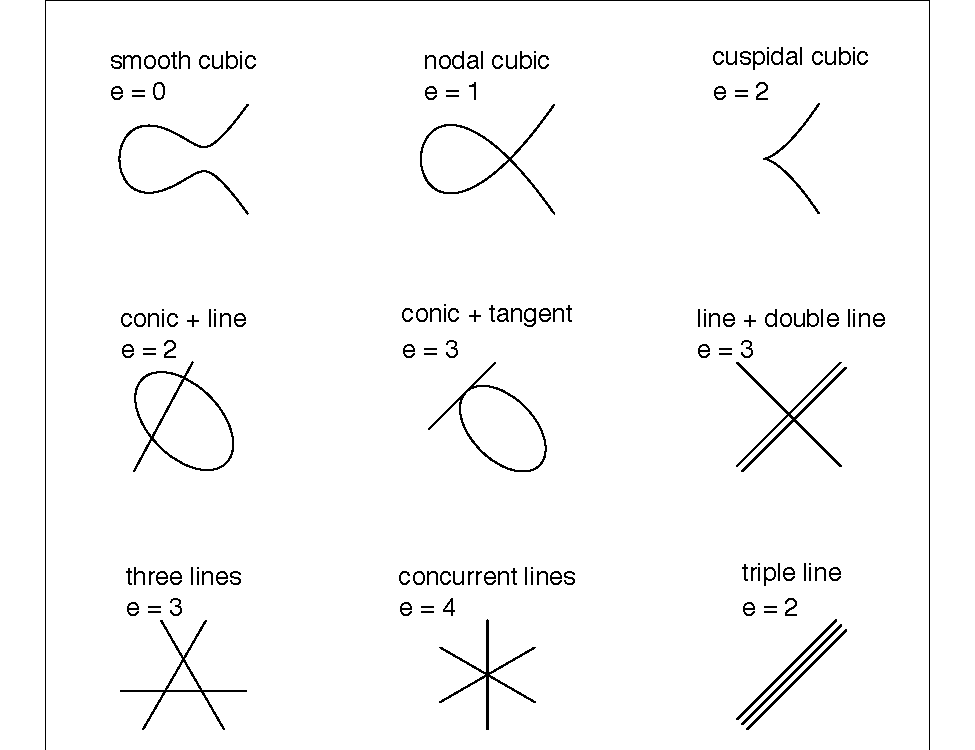
\includegraphics[width=1.0\textwidth]{planecubics}
  \caption{Cubic plane curves and their Euler characteristics \cite{Pic}}
\end{figure}

We may use tangent cones to differentiate the nodal cubics from singular cubics of other types. Suppose we find a singular point $Q$ of $C$. We ask two questions:
\begin{enumerate}
\item Does the tangent cone of $C$ at $Q$ contain a double line? If yes, then we have found a cuspidal cubic or a reducible cubic of the type conic + tangent, line + double line, or a triple line. 
\item Does the tangent cone of $C$ at $Q$ share an irreducible component, which has to be a line, with $C$? If yes, then we have found a reducible cubic. 
\end{enumerate}
If both answers are no, then we have found a nodal cubic. Now we explain how to perform the above tests using partial derivatives. 


Let us label the coordinates of $\IP^2$ as $X_0, X_1, X_2$ and let $Q \in \IP^2$ be a closed point. Without loss of generality, we assume $X_0(Q) \neq 0$ and dehomogenize a homogeneous cubic polynomial $g \in \kappa[X_0, X_1, X_2]$ at $X_0$ to a polynomial in $x_1 = X_1/X_0, x_2 = X_2/X_0$. The cubic $C = \{g = 0\}$ is singular at $Q$ if and only if 
$$ g(Q) = \frac{\p g}{\p x_1} (Q) = \frac{\p g}{\p x_2}(Q) = 0$$

Suppose $Q$ is a singularity. Note that $\deg Q$ has to be $1$ since a plane cubic cannot be singular at a point of higher degree. %In order for the conditions we shall impose on partial derivatives to be linear, we consider the projectivized tangent bundle $\IP(\sT_{\IA^2})$ of $\IA^2$, which is isomorphic to $\IP^1 \times \IA^2$. Let the homogeneous coordinates of the $\IP^1$ component by $U_0, U_1$. At each closed point $Q$, we may parametrize the lines through $Q$ by $U_0$ and $U_1$: 
% $$(U_0, U_1) \leftrightarrow U_1 (x_1 - x_1(Q)) + U_0(x_2 - x_2(Q)) =0 $$
For $m = 2, 3$, we define polynomials 
$$ T^m g(U_0, U_1) = \sum_{r + s = m} \frac{\p^m g}{\p x_1^r x_2^s}(Q) U_0^r U_1^s \in \kappa[U_0, U_1]$$
which are homogeneous in $U_0, U_1$. If $T^2 g(U_0, U_1) \equiv 0$, then the tangent cone of $C$ at $Q$ must have degree $3$, in which case $C$ must be a triple line, a line + double line, concurrent lines, or three lines. Otherwise, $T^2 g(x_1 - x_1(Q), x_2 - x_2(Q)) = 0$ describes the (affine) tangent cone of $C$ at $Q$, which we denote by $TC_Q(C)$. $TC_Q(C)$ contains a double line if and only if $T^2 g(U_0, U_1)$ vanishes at a closed point in $\IP^1 = \Proj \kappa[U_0, U_1]$ with multiplicity $\ge 2$. For convenience, we say a triple line contains a double line, and if $T^2 g(U_0, U_1) \equiv 0$, it vanishes at all points in $\Proj \kappa[U_0, U_1]$ with $\infty$ multiplicity. Taylor expansion of $g$ at $Q$ says
$$ g = T^2 g(x_1 - x_1(Q), x_2 - x_2(Q)) + T^3 g(x_1 - x_1(Q), x_2 - x_2(Q)) $$
we see that the $TC_Q(C)$ shares an irreducible component with $C$ if and only if there $T^2 g(U_0, U_1)$ and $T^3 g(U_0, U_1)$ share a zero on $\Proj \kappa[U_0, U_1]$. Therefore if we fix a particular closed point in $\Proj \kappa[U_0, U_1]$, then both conditions on $T^m(U_0, U_1)$ become linear in partial derivatives.

We may summarize the above observations into a geometric statement: Let $\IA^2 \subseteq \IP^2$ be the affine chart as above. Consider two subschemes of $\IA^2 \times \Proj \kappa[U_0, U_1]$: 
\begin{align*}
\sW_1 &= \{ g = \frac{\p g}{\p x_1} = \frac{\p g}{\p x_2} = T^2 g(U_0, U_1) = 0 \\
\sW_2 &= \{ g = \frac{\p g}{\p x_1} = \frac{\p g}{\p x_2} = T^2 g(U_0, U_1) = T^3 g(U_0, U_1) = 0 \} \\
\end{align*} 
\begin{enumerate}
\item If there does not exist a closed point $Q \in \IA^2$ such that the fiber of $\sW_1$ over $Q$ is non-reduced, then $C$ cannot be a cuspidal curve with the singularity in this affine chart $\IA^2$. 
\item If $\sW_2 = \emptyset$, then $C$ cannot be a reducible curve with a singularity in this affine chart $\IA^2$. 
\end{enumerate}
These statements are weaker than our observations, but they suffice for our purposes. We are going to use them in the proof of Lemma~\ref{elliptichigh}. 


\subsubsection{Counting Plane Cubics of Different Types}
In this section we count the number of reducible, cuspidal and nodal cubics in the projective plane $\IP^2$ over a finite field $\IF_q$. Plane cubics are given by sections in $S = H^0(\IP^2, \sO(3))$. We may identify $S$ with the subset of $\IF_q[X_0, X_1, X_2]$ consisting of homogeneous polynomials of degree $3$. Given $f \in S$, we denote its vanishing locus in $\IP^2$ by $Z(f)$. Define 
\begin{align*}
R &= \{ f \in S : Z(f) \textit{ is reducible} \} \\
C &= \{ f \in S : Z(f) \textit{ is cuspidal} \} \\
N &= \{ f \in S : Z(f) \textit{ is nodal} \}
\end{align*}

Let $H_j \subseteq \IF_q[U_0, U_1]$ denote the set of homogeneous polynomials of degree $j$. Given $g \in H_j$, denote its vanishing locus in $\IP^1 = \Proj \, \IF_q[U_0, U_1]$ by $Z(g)$. Note that $\dim_{\IF_q} H_j = j + 1$. If $g \in H_j$ and $W \in \IP^1$ is a finite subscheme, let $g|_W$ be the
element of $H^0(W, \sO_W)$ that on each connected component $W_i$ equals the restriction of $U_i^{-j} g$, where $i$ is the smallest index such that $U_i \neq 0$ at $W_i$. 
\begin{lemma} 
\label{square}
If $g_2 \in H_2, g_3 \in H_3$ are randomly chosen, then
$$ \Prob( g_2 \textit{ is coprime to } g_3 \, \mid \, g_2 \textit{ is a nonzero square}) =  1 - q^{-1}$$ 
\end{lemma}
\begin{proof}
Let $L$ be the closed point contained in $Z(g_2)$. $g_2$ and $g_3$ are coprime if and only if $L \not\in Z(g_3)$. Since $\deg L = 1$, the $\IF_q$-linear map $H_3 \to \kappa(L)$ given by $g_3 \mapsto g_3|_{L}$ is surjective. Therefore the probability that a randomly chosen $g_3 \in H_3$ vanishes at $L$ is $1/ \# \kappa(L) = 1/q$. 
\end{proof}

\begin{lemma}
\label{nonsquare} 
If $g_2 \in H_2, g_3 \in H_3$ are randomly chosen, then 
$$ \Prob(g_3 \textit{ is coprime to } g_2 \, | \, g_2 \textit{ is not a square}) = \frac{1}{q^3}(q + 1)(q - 1)^2 $$ 
\end{lemma}
\begin{proof}
Now we have to divide it into two cases. \\
\textit{Case 1:} $g_2$ is an reducible polynomial, so that $Z(g_2)$ contains two distinct closed points $L_1, L_2$, both of which have to be of degree $1$. $g_3$ is coprime to $g_2$ if and only if $L_1, L_2 \not\in Z(g_3)$. Since $H_3 \to \kappa(L_1) \oplus \kappa(L_2)$ is surjective, events $\{ g_3(L_1) = 0\} $ and $\{ g_3(L_2) = 0 \}$ are independent. Hence
$$\Prob(g_3 \textit{ is coprime to }g_2 \mid g_2 \textit{ is reducible}) = (1 - q^{-1})^2 $$ By counting the number of pairs $(L_1, L_2)$, $L_1 \neq L_2$, we easily see that 
$$ \# \{ g_2 \in H_2 : g_2 \textit{ is reducible with two distinct roots} \} = \frac{1}{2}q(q + 1)(q - 1)$$
where the factor $q - 1$ comes from the fact that $g_2$ is determined by $L_1, L_2$ up to scalar multiplication by $\IF_q^\times$. \\
\textit{Case 2:} $g_2$ is an irreducible polynomial. Then $g_3$ fails to be coprime to $g_2$ if and only if $g_2$ divides $g_3$ if and only if $g_3$ vanishes at $L_2:= Z(g_2)$, which is a closed point of degree $2$. Since $H_3 \to \kappa(L_2)$ given by $g_3 \mapsto g_3|_{L_2}$ is surjective, 
$$\Prob(g_3 \textit{ is coprime to }g_2 \mid g_2 \textit{ is irreducible}) = 1 - q^{-2} $$
Since there are $(q^2 - q)/2$ possible choices for $L_2$'s and $g_2$ is determined by $L_2$ up to a nonzero constant in $\IF_q$, we see that 
$$ \# \{ g_2 \in H_2 : g_2 \textit{ is irreducible} \} = \frac{1}{2}(q^2 - q)(q - 1)$$ 
Therefore the conditional probability in the lemma equals to 
$$ \frac{q + 1}{2q} (1 - q^{-1})^2 +  \frac{q - 1}{2q} (1 - q^{-2}) =  \frac{1}{q^3}(q + 1)(q - 1)^2 $$
\end{proof}

\begin{lemma}
\label{mainlemma}
Let $Q \in \IP^2$ be a closed point of degree $1$, then for a randomly chosen $f \in S$,
\begin{align*}
\Prob(f \textit{ is a cuspidal curve with a cusp at } Q) &= \frac{1}{q^7}(q - 1)^2(q + 1) \\
\Prob(f \textit{ is a nodal curve with a node at } Q) &= \frac{1}{q^7}(q - 1)^3(q + 1) \\
\end{align*} 
\end{lemma}
\begin{proof}
Without loss of generality, assume that $X_0 \neq 0$ at $Q$, so that $Q \in \IA^2$, on which we may use coordinates $x_1 = X_1/X_0, x_2 = X_2/X_0$. We further assume that $x_1(Q) = x_2(Q) = 0$, i.e. $Q$ is the origin of the affine chart $X_0 \neq 0$. We may identify $f \in S$ with its dehomogenization $f/X_0^3 = g(x_1, x_2)$ on $\IA^2$. We may write 
$$ g = g_0 + g_1 + g_2 + g_3 $$
where $g_j$ is the homogeneous part of degree $j$ of $g$. If $g_j$'s are chosen uniformly and independently at random, then the distribution of $f$ is uniform over $S$. $Z(g)$ is a cuspidal curve with a cusp at $Q$ if and only if 
\begin{enumerate}[i.]
\item $g_0 = g_1 = 0$ ($Z(f)$ is singular at $Q$.) 
\item $g_2 \neq 0$ and $g_2$ is a square. (The tangent cone of $Z(f)$ at $Q$ is a doubled line.)
\item $g_2$ and $g_3$ are coprime. ($Z(f)$ is irreducible.)
\end{enumerate} We easily see that $\Prob(i) = 1/q^3$, $\Prob(ii) = (q^2 - 1)/q^3$ and Lemma~\ref{square} gives $\Prob(iii \mid ii)$. Therefore the probability that $Z(f)$ has a cusp at $Q$ is 
$$ \frac{1}{q^3} \frac{q^2 - 1}{q^3} (1 - \frac{1}{q}) = \frac{1}{q^7}(q - 1)^2(q + 1) $$

Similarly, $Z(g)$ is a nodal curve with a node at $Q$ if and only if 
\begin{enumerate}[i.]
\item $g_0 = g_1 = 0$ ($Z(f)$ is singular at $Q$.) 
\item $g_2 \neq 0$ and $g_2$ is not a square. (The tangent cone of $Z(f)$ at $Q$ is two distinct lines.)
\item $g_2$ and $g_3$ are coprime. ($Z(f)$ is irreducible.)
\end{enumerate}
This time $\Prob(i) = 1/q^3$, $\Prob(ii) = (q^3 - q^2)/q^3$ and Lemma~\ref{nonsquare} gives $\Prob(iii \mid ii)$. Therefore the probability that $Z(f)$ has a node at $Q$ is 
$$ \frac{1}{q^3} \frac{q^3 - q^2}{q^3} \frac{1}{q^3}(q + 1)(q - 1)^2 = \frac{1}{q^7}(q - 1)^3(q + 1) $$
\end{proof}
\begin{lemma}
\begin{align*}
\# R &= (q^2 + q + 1)(q^6 - 1)\\
\# C &= q^3 (q^2 + q + 1) (q - 1)^2 (q + 1) \\
\# N &= q^3 (q^2 + q + 1) (q - 1)^3 (q + 1)
\end{align*}
\end{lemma}
\begin{proof}
We obtain the number $\# R$ from the obvious $(q - 1)$-to-$1$ surjection 
$$ (H^0(\IP^2, \sO(1)) - \{ 0 \}) \times (H^0(\IP^2, \sO(2)) - \{ 0 \}) \to R \subset H^0(\IP^2, \sO(3))$$
$\# C$ and $\# N$ follow directly from Lemma~\ref{mainlemma} and the facts that there are $(q^2 + q + 1)$ closed points of degree $1$ in $\IP^2$ over $\IF_q$ and $\dim_{\IF_q} S = 10$. 
\end{proof}

\subsection{Euler Characteristic}
Let $H_f \subseteq \IP^2 \times \IP^1$ be a non-singular hypersurface of bidegree $(3, d)$.  The Euler characteristic of $H_f$ tells us that $H_f$ will always contain some singular fibers with respect to the projection $\pi : H_f \to \IP^1$. Let $Z = \{ P \in \IP^1 : (H_f)_P \textit{ is singular }\}$, $Y^0 = H_f - \pi^{-1}(Z)$ and $X^0 = \IP^1 - Z$. Let $F$ denote a nonsingular cubic curve in $\IP^2$, which is unique up to isomorphism. We see that $Y^0$ is a $F$-bundle of $X^0$, and their Euler characteristics are related by 
$$ e(Y^0) = e(X^0 ) \cdot e(F) $$ 
Since $e(F) = 0$ we have that $e(Y^0) = 0$. Now since $H_f = Y^0 \coprod \pi^{-1}(Z)$, we see that $e(H_f) = e(Y^0) + e(\pi^{-1}(Z)) = e(\pi^{-1}(Z))$. Note that $C$ is a finite set of points, and hence $\pi^{-1} (Z)$ is a disjoint union of singular cubic curves. 

Now we compute $e(H_f)$. In fact we do a more general computation, since it is not harder. Let $H_f \subseteq \IP^2 \times \IP^1$ be a non-singular hypersurface of bidegree $(n, d)$. We denote the projections of $\IP^2 \times \IP^1$ onto the first and second components by $\pi_1, \pi_2$ respectively. Let $H_1$ be a hyperplane divisor of $\IP^2$ and $H_2$ be a hyperplane divisor of $\IP^1$. We define 
$$ A = \pi_1^*(H_1), \, E = \pi_2^*(H_2) $$
and $$ h_1 = A \cap H_f, \, h_2 = E \cap H_f $$
We compute the Chern classes of $H_f$ using the normal exact sequence:
$$ 0 \to T_{H_f} \to T_{\IP^2 \times \IP^1|_{H_f}} \to N_{H_f/\IP^2 \times \IP^1} \to 0$$
By Whitney product formula, their total Chern classes are related by
$$ c(T_{\IP^2 \times \IP^1|_{H_f}}) = c(T_{H_f}) c(N_{H_f/\IP^2 \times \IP^1}) $$
Now $T_{\IP^2 \times \IP^1|_{H_f}}$ is $T_{\IP^2 \times \IP^1} = \pi_1^* T_{\IP^2} \oplus \pi_2^* T_{\IP^1}$ restricted to $H_f$, so we obtain 
$$ c(T_{\IP^2 \times \IP^1|_{H_f}}) = (1 + 3h_1 + 3h_1^2)(1 + 2h_2) $$
If $\iota : H_f \into \IP^2 \times \IP^1$ is the inclusion, then $$N_{H_f/\IP^2 \times \IP^1} = \iota^* \sO_{\IP^2 \times \IP^1}(nA  + dE) = (1 + nh_1 + dh_2)$$
Therefore 
\begin{align*}
c(T_{H_f}) &= c(T_{\IP^2 \times \IP^1|_{H_f}})c(N_{H_f/\IP^2 \times \IP^1})^{-1}\\
&= (1 + 3h_1 + 3h_1^2)(1 + 2h_2)(1 + nh_1 + dh_2)^{-1}\\
&= (1 + 3h_1 + 3h_1^2)(1 + 2h_2)(1 - (nh_1 + dh_2) + (nh_1 + dh_2)^2 - \cdots)
\end{align*}
In particular we obtain 
$$ c_2(T_{H_f}) = (n^2 - 3n + 3)h_1^2 + (6 + 2nd - 2n - 3d)h_1 h_2 $$
which is the top Chern class. Now we compute 
\begin{align*}
\deg h_1^2 &= A \cdot A \cdot (nA + dE) = d \\
\deg h_1 h_2 &= A \cdot E \cdot (nA + dE) = n 
\end{align*}
Finally we obtain 
$$ e(H_f) = \deg c_2(T_{H_f}) = 6n + 3d + 3n^2 d - 6 dn - 2n^2 $$
In particular, for future use we want to fix $n = 3$, so $e(H_f)$ depends only on $d$. In this case $e(H_f) = 12 d$. 

We note that if all singular fibers of $H_f$ are nodal, then $e(H_f)$ is exactly the number of singular fibers. Therefore this answer should be expected: when $d = 1$, $H_f$ corresponds to a copy of $\IP^1$ in $\IP H^0(\IP^2, \sO(3))$ cut out by hyperplanes, and the degree of the determinantal locus that parametrizes singular cubics is $12$.  

\subsection{A Density Result over Finite Fields}
In a similar vein as in section~\ref{simplify-ramified}, we are going to work with the following sets:
For a fixed $e_0 \in \IN$, we define 
\begin{align*}
\sP_{e_0}^{\mathrm{low}} &= \union_{d \ge 0} \{ f \in S_{n, d} : H_f \textit{ is good at all $P \in \IP^1_{\IF_q}$,}\deg P < e_0\}\\
\sQ_{e_0}^{\mathrm{med}} &= \union_{d \ge 0} \{f \in S_{n, d} : H_f \textit{ is bad at some $P \in \IP^1_{\IF_q}$,}\deg P \in [e_0, \lfloor d/p \rfloor]\}\\
\sQ^{\mathrm{high}} &= \union_{d \ge 0} \{f \in S_{n, d} : H_f \textit{ is bad at some $P \in \IP^1_{\IF_q}$,}\deg P \in > d/p\}
\end{align*}
\subsubsection{Points of Low and Medium Degree}
 

We first do some local analysis on a fiber. Let $P \in \IP^1$ be a fixed point and let $e = \deg P$. Let $r(s) \in \IF_q[s]$ be an irreducible polynomial such that the second infinitesimal neighborhood $P^{(2)} = \Spec \IF_q[s]/r(s)^2$. Let $B := \IF_q[s]$ and $\fm := (r(s)) \subseteq B$ be the maximal ideal. Denote the restriction map $B/\fm^2 \to B/\fm$ by $g \mapsto \overline{g}$ and extend it to a map $H^0(\IP^2_{B/\fm^2}, \sO(3)) \to H^0(\IP^2_{B/\fm}, \sO(3))$ by applying the reduction map to each coefficient. Similarly we denote a $\IF_q$-linear section of the reduction map $B/\fm^2 \to B/\fm$ by $h \to \wt{h}$\footnote{I want to specify this map as: for each $f \in B/\fm$ there is a unique representative with degree $\le \deg r(s)$, interpret it as an element in $B/\fm^2$.} and extend it to a map $H^0(\IP^2_{B/\fm}, \sO(3)) \to H^0(\IP^2_{B/\fm^2}, \sO(3))$. Let $\varphi_P : S_{3, d} \to H^0(\IP^2_{B/\fm^2}, \sO(3))$ be the restriction map. $H_f$ is non-singular at a point $Q \in \pi^{-1}(P)$ if and only if $\varphi_P(f)$ does not vanish at $Q^{(2)} \in \IP^2_{B/\fm^2}$. 


Consider the vector space $H^0(\IP^2_{\IF_{q^e}}, \sO(3))^2$, we say that a pair $(F_1, F_2)$ is good if, it satisfies one the following conditions:
\begin{enumerate}
\item $F_1$ describes a non-singular curve in $\IP^2_{\IF_{q^e}}$.
\item $F_1$ describes a nodal curve but $F_2$ does not vanish at the node.
\end{enumerate}  
This terminology is explained by the following lemma, which is an analogous statement to Lemma~\ref{pair}. 
\begin{lemma}
\label{conversion}
The map
$$ \varphi : H^0(\IP^2_{B/\fm} , \sO(3))^2 \to H^0(\IP^2_{B/\fm^2}, \sO(3))$$ defined by 
$$ (F_1, F_2) \mapsto \wt{F_1} + r(s) F_2 $$
is an isomorphism of vector spaces. Moreover, $f$ is good at $P$ if and only if $\varphi_P(f)$ in $H^0(\IP^2_{B/\fm} , \sO(3))^2$ is a good pair. 
\end{lemma}
\begin{proof}
The above map has an inverse $F \mapsto (\overline{F}, (F - \wt{\overline{F}}))/r(s))$. For $f$ to be good at $P$, we need $\overline{\varphi_P(f)}$ to describe a non-singular or nodal curve. Let $Q \in \IP^2_{B/\fm^2}$ be a closed point and suppose $\varphi_P(f)$ corresponds to $(F_1, F_2)$. If $F_1$ is non-singular at $Q$, then $H_f$ must also be non-singular at $Q$. Otherwise, $H_f$ is non-singular at $Q$ if and only if $F_2$ does not vanish at $Q$. 
\end{proof}

The following lemma assumes the same role as lemma~\ref{Low} as in Section~\ref{simplify-ramified}, and the proof is similar. 
\begin{lemma}
\label{pointsurj}
If $\{P_1, P_2, \cdots, P_s\}$ is a set of finitely many closed points in $\IP^1$, then for $f$ randomly chosen from $\union_d S_{3, d}$,
$$ \Prob(f \textit{ is good at all } P_i) = \prod_{i = 1}^s \Prob( f \textit{ is good at all points } P_i) $$
In particular, we have
$$\Prob(f \in \sP_{e_0}^{\mathrm{low}})  = \prod_{\deg(P) < e_0}  \Prob( f \textit{ is good at all points } P ) $$
since there are only finitely many points with degree $< e_0$. 
\end{lemma}
\begin{proof} 
Denote $\IP^2 \times \IP^1$ by $X$. Let $W := \coprod P_i^{(2)}$ and $\delta := \deg W = \sum_{i = 1}^s 2 \deg P_i$. Then we have an exact sequence 
$$ 0 \to \sO_X(3, d - \delta) \to \sO_X(3, d) \to \sO_X(3, d)|_{X_W} \to 0  $$
which induces an exact sequence 
$$ H^0(X, \sO_X(3, d)) \to H^0(X_W, \sO_X(3, d)|_{X_W}) \to H^1(X, \sO_X(3, d - \delta)) $$
By K{\"u}nneth formula, 
$$ H^1(X, \sO_X(3, d - \delta)) \iso \bigoplus_{i + j = 1} H^i(\IP^2, \sO(3))\tensor_{\IF_q} H^j(\IP^1, \sO(d - \delta))   $$
However, when $d - \delta \ge 0$, Lemma 29.8.1 in \cite[Tag 01XS]{stacks-project} implies $H^1(\IP^2, \sO(3)) = H^1(\IP^1, \sO(d - \delta)) = 0$. 
Therefore $H^1(X, \sO_X(3, d - \delta)) = 0$ and the restriction map
\begin{align*}
S_{3, d} = H^0(\IP^2 \times \IP^1, \sO(3, d)) \to H^0(X_W, \sO_X(3, d)|_{X_W}) \cong \prod_{i = 1}^s H^0(X_{P_i^{(2)}}, \sO(3))
\end{align*}
is surjective for $ d \ge \sum_i 2 \deg P_i$. This surjectivity, together with our observation that whether $f$ is good at all $Q \in (H_f)_{P_i}$ is completely determined by $\varphi_{P_i}(f) \in H^0(\IP^1_{P_i^{(2)}}, \sO(3))$, implies that when $d \ge \delta$, we have 
$$ \frac{\# S_{3, d} \cap \sP_{e_0}^{\mathrm{low}}}{\# S_{3, d}} = \prod_{i = 1}^s \frac{\# \varphi_{P_i}(\{ f \in S_{3, d} : f \textit{ is good at }P_i\})}{\# H^0(X_{P^{(2)}_i}, \sO(3))} $$
The lemma follows by taking $d \to \infty$ on both sides. 
\end{proof}

\begin{lemma}
\label{prepcount}
The fraction of good pairs in $H^0(\IP^2_{\IF_{q^e}}, \sO(3))^2$ is $$(1 + q^{-2e})(1 - 2q^{-2e} - q^{-4e} + q^{-5e} - 2q^{-6e} -q^{-7e})$$ 
By the previous lemma, if $e = \deg P$, then this fraction is precisely $\Prob(f \in \sS_P)$.
\end{lemma}
\begin{proof}
A randomly chosen $(F_1, F_2) \in H^0(\IP^2_{\IF_{q^e}}, \sO(3))^2$ fails to be good if and only if one of the following four events happen:
\begin{enumerate}
\item $F_1$ describes a nodal curve, and $F_2$ vanishes at the node of $F_1$. 
\item $F_1$ describes a cuspidal curve. 
\item $F_1$ describes a reducible curve. 
\item $F_1 \equiv 0$. 
\end{enumerate} 
We denote the above events by $E_1, E_2, E_3, E_4$ respectively. To simplify notation, we denote $q^e$ by a bold $\pmb{q}$. Our results on the number of cubics of different types readily imply 
\begin{align*}
\Prob(E_1) &= \Prob(F_1 \textit{ is a nodal curve})\Prob(F_2 \textit{ vanishes at the node of } F_1) \\
&= \frac{1}{\pmb{q}^7}(\pmb{q}^2 + \pmb{q} + 1) (\pmb{q} - 1)^3 (\pmb{q} + 1) \cdot \frac{1}{\pmb{q}} \\
&= \frac{1}{\pmb{q}^8}(\pmb{q}^2 + \pmb{q} + 1) (\pmb{q} - 1)^3 (\pmb{q} + 1)
\end{align*}
and 
\begin{align*}
\Prob(E_2) &= \frac{1}{\pmb{q}^7} (\pmb{q}^2 + \pmb{q} + 1) (\pmb{q} - 1)^2 (\pmb{q} + 1)\\
\Prob(E_3) &= \frac{1}{\pmb{q}^{10}} (\pmb{q}^2 + \pmb{q} + 1)(\pmb{q}^6 - 1)
\end{align*}
It is clear that $\Prob(E_4) = \pmb{q}^{-10}$. The events $E_j$'s are clearly disjoint, so the fraction of good pairs in the lemma is computed by 
$$ 1 - \sum_{j = 1}^4 \Prob(E_j) $$
\end{proof}

\noindent \textit{Proof of Lemma~\ref{pcount}}. Lemma~\ref{conversion} and \ref{pointsurj} implies that $\mu(\sS_P)$ is precisely the fraction of good pairs in $H^0(\IP^2_{\IF_{q^e}}, \sO(3))^2$, which is computed in Lemma~\ref{prepcount}. \qed



\subsubsection{Points of High Degree}
We are going to bound the probability that a randomly chosen $f \in S_{3, d}$ is bad at some point $P$ with high degree $(> \lfloor d/p \rfloor)$. Therefore the following lemmas is to be applied with $j = \lfloor d/p \rfloor$. The main idea used here has been explained in section~\ref{classification}.

Let $A_{3, d} = \IF_q[x, y]\tensor_{\IF_q} \IF_q[t]$. 
%and $\sB \subseteq \union_d A_{3, d}$ be a subset. We say that the (asymptotic) probability that a randomly chosen $f \in A_{3, d}$ lies in $\sB$ is 
%$$ \lim_{d \to \infty} \frac{\# \sB \cap A_{3, d}}{\# A_{3,d}} $$
For each $f \in A_{3, d}$ we define polynomials
\begin{align*}
T^2 f(U_0, U_1, x, y, t) &= f_{xx}U_1^2 + 2f_{xy} U_1 U_0 + f_{yy} U_0^2 \\
T^3 f(U_0, U_1, x, y, t) &= f_{xxx} U_1^3 + 3 f_{x^2 y} U_1^2 U_0 + 3 f_{x y^2} U_1 U_0^2 + f_{y^3} U_0^3 
\end{align*}


\begin{lemma}
\label{elliptichigh}
Let $U$ be an open subscheme of $\IP^2 \times \IP^1$ and $j > 2$ be an integer. The probability that for a randomly chosen $f \in S_{3, d}$ such that there exists a closed point $Q \in U$ that satisfies the following two conditions
\begin{enumerate}
\item $P := \pi(Q)$ has degree $> j$. 
\item The fiber $(H_f)_P$ is a cuspidal or reducible cubic with a singularity at $Q$, or the hypersurface $H_f$ has a singularity at $Q$. 
\end{enumerate}
is bounded by 
$$ O(d^4 q^{-\min(\lfloor d/p \rfloor + 1, j)}) $$
\end{lemma}

\begin{proof}
It suffices to show the lemma for an affine chart $\IA^2 \times \IA^1$ since $\IP^2 \times \IP^1$ can be covered by six such charts. Without loss of generality, assume that $X_0, T_0 \neq 0$ on $U = \IA^2 \times \IA^1$ and let $x = X_1/X_0, y = X_2/X_0$ and $t = T_1/T_0$, such that $U = \Spec \IF_q[x, y] \tensor_{\IF_q} \IF_q[t]$. (Identify $S_{3, d}$ with $A_{3, d}$). Following the ideas presented in section~\ref{classification}, it suffices to bound the density of $f \in A_{3, d}$ such that there exists a closed point $Q \in \IA^2 \times \IA^1$ that satisfies the following three conditions
\begin{enumerate}
\item $P := \pi(Q)$ has degree $> j$. 
\item $f(Q) = f_x(Q) = f_y(Q) = 0$
\item $T^2 f(U_0, U_1, Q)$ and $T^3 f(U_0, U_1, Q)$ have a common zero on $\Proj \IF_q[U_0, U_1]$ (\textbf{Type \uppercase\expandafter{\romannumeral1}}), $T^2 f(U_0, U_1, Q)$ vanishes at a point on $\Proj \IF_q[U_0, U_1]$ with multiplicity $\ge 2$ (\textbf{Type \uppercase\expandafter{\romannumeral2}}), or $f_t(Q) = 0$ (\textbf{Type \uppercase\expandafter{\romannumeral3}}).
\end{enumerate}

To bound the density of polynomials of Type \uppercase\expandafter{\romannumeral1} or Type \uppercase\expandafter{\romannumeral2}, we are naturally led to consider the scheme $\Proj \IF_q[U_0, U_1] \times \IA^2 \times \IA^1$. \\\\
\textbf{Type \uppercase\expandafter{\romannumeral1}: } $f$ is of Type I only if there exists a closed point $Q'$ in the subscheme
$$ W_0 := \{f = f_x = f_y = T^2 f = T^3 f = 0\} \subseteq \Proj \IF_q[U_0, U_1] \times \IA^2 \times \IA^1 $$
such that $\deg \pi(Q') \ge j$, where we still denote the projection to the last $\IA^1$ component by $\pi$. 

On the affine chart $U' = \Spec \IF_q[u] \times \IA^2 \times \IA^1$ where $u = U_1/U_0$, we dehonogenize $T^2 f, T^3 f$ to:
\begin{align*}
T^2 f(u, x, y, t) &= f_{xx} u^2 + 2 f_{xy} u + f_{yy} \\
T^3 f(u, x, y, t) &= f_{xxx} u^3 + 3 f_{x^2 y} u^2 + 3 f_{xy^2}u + f_{yyy} 
\end{align*}

We call a point $Q' \in \Proj \IF_q[U_0, U_1] \times \IA^2 \times \IA^1$ \textit{admissible} if $\deg \pi(Q) \ge j$ and a subscheme $V$ \textit{admissible} if it contains an admissible point. By $(V)_\ad$ we denote the union of admissible irreducible components of $(V)_{\mathrm{red}}$. 


Following Poonen's idea, we write $f$ in a form so that the derivatives involved are largely independent. If $h \in A_{3, d}$, $g_i \in A_{0, \yk}$ for $0 \le i \le 4$ uniformly and independently at random, then the distribution of 
$$ f = h + g_4^p x^3  + g_3^p y^2 + g_2^p x + g_1^p y + g_0^p  $$ 
is also uniform over $A_{3, d}$. 
Direct computation shows 
\begin{align*}
T^3 f &= u^3(h_{xxx} + 6 g_4^p) + 3 u^2 h_{x^2 y} + 3 u h_{xy^2} + h_{yyy} \\
T^2 f &= u^2(h_{xx} + 6x g_4^p) + 2 u h_{xy} + h_{yy} + 2 g_3^p \\
f_x &= h_x + 3 g_4^p x^2 + 2 g_3^p x + g_2^p \\
f_y &= h_y + g_1^p
\end{align*}
We define a sequence of subschemes $W_4 \subseteq \cdots \subseteq W_0 \subseteq U$ by 
\begin{align*}
W_4 &= \{ T^3 f = 0 \}, W_3 = W_4 \cap \{ T^2 f = 0 \} \\
W_2 &= W_3 \cap \{ f_x = 0 \}, W_1 = W_2 \cap \{ f_y = 0 \}
\end{align*}
As the reader may check, we deliberately set up the supscripts so that for each $k = 0,\cdots, 4$, $W_k$ only depends on the choice of $h, g_{k}, \cdots, g_4$. Let $E$ denote the event that 
\begin{enumerate}[a.]
\item $\dim (W_1)_\ad = 0$
\item $f$ does not vanish at any of $\Irr (W_1)_\ad$. 
\end{enumerate} 
Clearly if $E$ holds for $f$, then $W_0$ does not contain any admissible point. Therefore it suffices to show that for randomly chosen $h, g_1, \cdots, g_4$,
$$ \Prob(E) = 1 - O(d^4 q^{- \min(\yk + 1, j)})$$
\textit{Step 1:} Conditioned on a choice of $h$, the probability that $\dim W_4 = 4$ is at most $q^{-(\yk + 1)}$. \\
\textit{Proof of Step 1: }Indeed, $\dim W_4 = 4$ if only if $T^3 f$ vanish identically on $U$, which happens only when $T^3 f = 0$ as a polynomial in $\IF_q[u, x, y, t]$, and in particular $h_{xxx} + 6 g_4^p = 0$. For each $h$, there is at most one choice for $g_4$ such that $h_{xxx} + 6 g_4^p = 0$, and hence the claim follows. \\\\
\textit{Step 2:} For $k = 3, 2, 1$, conditioned on a choice of $h, g_k, \cdots, g_4$ for which $\dim W_{k + 1} \le k$, the probability that $\dim (W_k)_\ad \ge k$ is at most $O(d^{4 - k} q^{- \min(\yk + 1, j)})$.\\
\textit{Proof of Step 2: }We only show this for $k = 3$, since the proofs for $k = 2, 1$ are completely analogous. Let $V_1, \cdots, V_\ell$ be all the irreducible components of $(W_4)_\ad$, where $\ell = \# \{\Irr (W_4)_\ad \}$. By B{\`e}zout's theorem, $\ell = O(d)$. We need to bound the set 
$$ G_i^{\mathrm{bad}} = \{ g_3 \in A_{0, \yk} : T^2 f \textit{ vanishes identically on }V_i \} $$ 
If $g, g' \in G_i^{\mathrm{bad}}$, then $g - g'$ vanishes identically on $V_i$. Hence if $G_i^{\mathrm{bad}} \neq \emptyset$, it is a coset of the kernel of the linear map 
$$ \varphi_i : A_{0, \yk} \to H^0(V_i, \sO_{V_i}) $$ 
Now we apply Lemma~\ref{prep} by identifying $U' = \IA^1 \times \IA^2 \times \IA^1$ with $\IA^3 \times \IA^1$ to obtain that $\# \{ \im \varphi_i \} \ge q^{\min(\yk + 1, j)}$. Therefore the probability that a randomly chosen $g_3$ lies in $G_i^{\mathrm{bad}}$ is at most  $q^{- \min(\yk + 1, j)}$. Since there are $O(d)$ such $V_i$'s, the claim follows. \\\\
\textit{Step 3: }Conditioned on choice $h, g_4, \cdots, g_1$ such that $\dim (W_1)_\ad = 0$, the probability that $(W_0)_\ad \neq \emptyset$ is at most $O(q^4 q^{- \min(\yk + 1, j)})$. \\
\textit{Proof of Step 3:} By B{\`e}zout's theorem again, we see that $\# \{ W_0 \} = O(d^4)$. For an admissible point $Q \in W_0$, the set $H^{\mathrm{bad}}$ of $g_0 \in A_{0, \yk}$ for which $f$ vanishes at $Q$ forms a coset of the kernel of the map $\varphi_Q : A_{0, \yk} \to H^0(Q, \sO_Q)$. We apply Lemma~\ref{prep} again with $W = Q$ to prove claim 3. \\
Finally \textit{Step 1} and \textit{2} combined to give that 
\begin{align*}
\Prob(\dim (W_1)_\ad) = 0) &\ge (1 - q^{-(\yk + 1)})\prod_{k = 1}^3 (1 - d^k q^{- \min(\yk + 1, j)}) \\
&= 1 - O(d^3 q^{- \min(\yk + 1, j)})
\end{align*}
and \textit{Step 3} gives 
\begin{align*}
\Prob(E) &\ge \Prob(\dim (W_1)_\ad) = 0)( 1 - O(d^4 q^{- \min(\yk + 1, j)}) \\ 
&= 1 - O(d^4 q^{- \min(\yk + 1, j)})
\end{align*}
\textbf{Type \uppercase\expandafter{\romannumeral2}}: We can check whether $f$ is of Type \uppercase\expandafter{\romannumeral2} locally. It suffices to bound the density of $f \in A_{3, d}$ such that there exists a closed point $Q' \in U'$ in the subscheme 
$$ W_0' = \{ f = f_x = f_y = T^2 f = (T^2 f)_u = 0 \} \subseteq U' $$
with $\deg \pi(Q') \ge j$. 
The rest of the arguments is rather analogous to what we did before, so we only give a sketch. We define 
\begin{align*}
W'_4 &= \{ (T^2 f)_u = 0 \}, W'_3 = W_4' \cap \{ T^2 f = 0 \} \\
W'_2 &= W'_3 \cap \{ f_x = 0 \}, W'_1 = W'_2 \cap \{ f_y = 0 \}
\end{align*}
This time we choose $f \in A_{3, d}$ by choosing $h \in A_{3, d}$, $g_i \in A_{0, \yk}$ for $0 \le i \le 4$ uniformly and independently at random and putting 
$$ f = h + g_4^p xy + g_3^p y^2 + g_2^p x + g_1^p y + g_0^p $$
Direct computation shows 
\begin{align*}
(T^2 f )_u &= 2u h_{xx} + 2(h_{xy} + g_4^p) \\
T^2 f &= u^2 h_{xx} + 2 u (h_{xy} + g_4^p) + h_{yy} + g_3^p \\
f_x &= h_x + g_4^p y + g_2^p \\
f_y &= h_y + g_1^p 
\end{align*}
By applying the same argument as in \textit{Step 1} and \textit{2}, we may show that 
$$ \Prob(\dim(W'_1)_\ad = 0) = 1 - O(d^3 q^{- \min(\yk + 1, j)}) $$
By applying the same arguments as in \textit{Step 3}, we may bound the probability that $f$ does not vanish at any of the irreducible components of $(W_2')_\ad$ given than $\dim (W'_2)_\ad = 0$, so that 
$$ \Prob((W_0')_\ad = \emptyset) \ge 1 - O(d^4 q^{- \min(\yk + 1, j)}) $$\\\\
\textbf{Type \uppercase\expandafter{\romannumeral3}}: This is the easiest case to deal with. There is no need to involve $U_i$'s. The proof is completely analogous to the second part of the proof of Lemma~\ref{prep}, where we treated the case in which the curve $H_f$ has a singularity on $\IA^1 \times \IA^1$, except that we have $\IA^2 \times \IA^1$ instead of $\IA^1 \times \IA^1$ and one more variable in this case. \\\\ 
Now the proof of the lemma is complete. 
\end{proof}

\subsubsection{Proof of the Main Result}
\begin{lemma}
\label{ellipticmed}
$$ \lim_{e_0 \to \infty} \Prob( f \in \sQ_{e_0}^{\mathrm{med}}) = 0 $$
\end{lemma}
\begin{proof}
By definition, 
$$ \Prob( f \in  \sQ_{e_0}^{\mathrm{med}}) = \lim_{d \to \infty} \Prob(f_d \in \sQ_{e_0}^{\mathrm{med}})$$
for $f_d$ randomly chosen from $S_{3, d}$. It suffices to show that $\Prob(f_d \in \sQ_{e_0}^{\mathrm{med}})$ is universally bounded by $O(q^{-e_0})$, where the implied constant is independent of $d$ or $e_0$. 

Let $P$ be a point of degree $e \le \lfloor d/p \rfloor$ on $\IP^1$. By the proof of Lemma~\ref{pointsurj}, the restriction map $S_{3, d} \to H^0(X_{P^{(2)}}, \sO(3))$ is surjective since $p > 2$ and $e < \lfloor d/p \rfloor < d/2$. Lemma~\ref{pair} and Lemma~\ref{pcount} hence imply that probability that $f_d$ is bad at $P$ is $O(q^{-2e})$ as $e \to \infty$. 
\begin{align*}
\Prob(f_d \in \sQ_{e_0}^{\mathrm{med}}) &\le \sum_{e = e_0}^{\lfloor d/p \rfloor} (\text{number of points of degree $e$ in $\IP^1$})(2q^{-2e}) \\
&\le 2 \sum_{e = e_0}^{\lfloor d/p \rfloor}(q^{e} + 1) q^{-2e} = O(\frac{q^{-e_0}}{1 - q^{-1}}) = O(q^{-e_0})
\end{align*} 
\end{proof}

\begin{lemma}
\label{elliptichighf}
$$ \Prob(f \in \sQ^{\mathrm{high}}) = 0 $$
\end{lemma}
\begin{proof}
Apply Lemma~\ref{elliptichigh} with $j = \fl{d/p}$ and $U = \IP^2 \times \IP^1$. Then push $d \to \infty$. 
\end{proof}

For each $e_0$, we have 
$$ \sP_{e_0}^{\mathrm{low}} \subseteq \sS \subseteq \sP_{e_0}^{\mathrm{low}} \cup \sQ_{e_0}^{\mathrm{med}} \cup \sQ^{\mathrm{high}}$$
As $e_0 \to \infty$, Lemma~\ref{pointsurj}, \ref{ellipticmed} and \ref{elliptichighf} combine to give that 
$$ \Prob(f \in \sS) = \prod_{P \in \IP^1_{\IF_q}} \Prob( f \in \sS_P) $$

Recall the following well known lemma:
\begin{lemma}
Suppose that $p_e, e = 1, 2, \cdots$ satisfy $0 \le p_e < 1$ and $\sum p_e < \infty$, then $\prod (1 - p_e) > 0$. 
\end{lemma}
By Lemma~\ref{pcount}, the infinite product 
$$ \prod_{P \in \IP^1_{\IF_q}} \Prob( f \in \sS_P) = \prod_{e = 1}^\infty (\prod_{\deg P = e} \Prob(f \in \sS_P))$$
converges since 
$$ 1 - \prod_{\deg P = e} \Prob(f \in \sS_P) \le O(q^{-e})$$

\begin{thebibliography}{9}
\bibitem{expository}
B. Poonen, \textit{Sieve methods for varieties over finite fields and arithmetic schemes}, J. Théor. Nombres Bordeaux 19 (2007), 221–229.

\bibitem{Pic}
B. Poonen, \textit{An explicit algebraic family of genus-one curves violating the Hasse principle}, available at \url{http://www-math.mit.edu/~poonen/}, 

\bibitem{Wood}
D. Erman and M.M. Wood, \textit{Semiample Bertini theorems over finite fields}, Duke Mathematical Journal 164(2015), no. 1, 1-38

\bibitem{Poonen}
B. Poonen, \textit{Bertini theorems over finite fields}, Ann. of Math. (2) 160 (2004), no. 3, 1099-1127.

\bibitem{Hartshorne}
Robin Hartshorne, \textit{Algebraic geometry}, Springer-Verlag, New York, 1977, Graduate Texts in
Mathematics, No. 52.

\bibitem{stacks-project}
The Stacks Project Authors, \textit{Stacks Project}, \url{http://stacks.math.columbia.edu}, 2016


\end{thebibliography}




\end{document}